% !TEX program = xelatex
% ============================================================
%  计算机图形学实验报告（合并版 · 8 个实验）
%  作者：张致远  学号：2023213980  班级：信计23-1  指导教师：霍鑫
%  编译方式：xelatex report_template.tex （连续运行两次以稳定页眉/页码/目录）
%
%  文档结构：
%    \section{实验一 / 实验二 / ... / 实验八}
%        \subsection{实验目的}
%        \subsection{实验要求}
%        \subsection{关键算法及实现原理}
%        \subsection{程序调试中的问题}
%        \subsection{程序运行结果或数据}
%        \subsection{实验收获及体会}
%    \section{实验代码}
%        \subsection{实验一代码}
%        \subsection{实验二代码}
%        ...
% ============================================================

\documentclass[a4paper,12pt]{ctexart}

% ---------- 页面与页眉 ----------
\usepackage[a4paper,left=2.5cm,right=2.5cm,top=2.5cm,bottom=2.5cm]{geometry}
\usepackage{fancyhdr}
\setlength{\headheight}{14.5pt}
\pagestyle{fancy}
\fancyhf{}
\fancyhead[L]{计算机图形学实验报告}
\fancyhead[R]{\nouppercase{\leftmark}}
\fancyfoot[C]{\thepage}
\renewcommand{\headrulewidth}{0.4pt}

% ---------- 通用宏包 ----------
\usepackage{array}
\usepackage{booktabs}
\usepackage{graphicx}
\usepackage{xcolor}
\usepackage{amsmath,amssymb}
\usepackage{caption}
\usepackage{enumitem}
\usepackage{float}
\usepackage{hyperref}
\hypersetup{
    colorlinks=true,
    linkcolor=black,
    urlcolor=blue,
    pdftitle={计算机图形学实验报告},
    pdfauthor={张致远}
}

% ---------- 代码环境 ----------
\usepackage{listings}
\definecolor{codegray}{rgb}{0.5,0.5,0.5}
\definecolor{codegreen}{rgb}{0,0.5,0}
\definecolor{codepurple}{rgb}{0.58,0,0.82}
\definecolor{codebg}{rgb}{0.97,0.97,0.97}
\lstset{
    backgroundcolor=\color{codebg},
    basicstyle=\ttfamily\small,
    commentstyle=\color{codegreen}\itshape,
    keywordstyle=\color{blue}\bfseries,
    stringstyle=\color{codepurple},
    numberstyle=\tiny\color{codegray},
    numbers=left,
    numbersep=8pt,
    frame=single,
    rulecolor=\color{black!30},
    breaklines=true,
    breakatwhitespace=true,
    showstringspaces=false,
    tabsize=4,
    captionpos=b,
    xleftmargin=1em,
    xrightmargin=1em,
    columns=flexible
}
\lstdefinestyle{cppstyle}{language=C++}

% ---------- 章节标题外观 ----------
\ctexset{
    section/format = \Large\bfseries\heiti,
    subsection/format = \large\bfseries\heiti,
    subsubsection/format = \normalsize\bfseries\heiti
}

% ============================================================
\begin{document}

% ============================================================
%  封面（仅一次）
% ============================================================
\thispagestyle{empty}
\begin{center}
    \vspace*{2cm}
    {\zihao{-0}\heiti 计算机图形学\\[0.4em]实验报告}\\[3cm]

    \renewcommand{\arraystretch}{1.8}
    {\zihao{3}
    \begin{tabular}{r@{\quad}l}
        \textbf{姓\hspace{2em}名：} & 张致远 \\
        \textbf{学\hspace{2em}号：} & 2023213980 \\
        \textbf{专业班级：}         & 信计 23-1 \\
        \textbf{指导教师：}         & 霍\,\,星 \\
        \textbf{完成日期：}         & 2026 年 5 月 9 日 \\
    \end{tabular}}
    \vfill
\end{center}
\clearpage

% ============================================================
%  目录
% ============================================================
\thispagestyle{plain}
\tableofcontents
\clearpage

% ============================================================
%  ============== 实验一  直线的生成 ==============
% ============================================================
\section{实验一\quad 直线的生成}

\subsection{实验目的}

\begin{enumerate}[leftmargin=2em,itemsep=0.2em]
    \item 理解光栅图形系统中直线段扫描转换的基本思想，体会"用离散像素逼近连续直线"这一图形学核心问题。
    \item 掌握 DDA 算法、中点画线算法以及 Bresenham 算法的数学推导与实现细节。
    \item 通过对三种算法的实现与比较，分析它们在效率、误差、可移植性等方面的差异，重点掌握 \textbf{Bresenham 直线生成算法} 的递推逻辑。
    \item 熟悉 OpenGL 编程基本框架，能够利用 \texttt{GL\_POINTS} 模式按算法逐像素绘制图元。
\end{enumerate}

\subsection{实验要求}

\textbf{实验环境：}
\begin{itemize}[leftmargin=2em,itemsep=0.2em]
    \item 实验设备：PC 机一台
    \item 操作系统：Windows 11
    \item 开发工具：Visual Studio 2022 + OpenGL（freeglut 3.4.0）
    \item 编程语言：C++
\end{itemize}

\textbf{实验内容：}
\begin{enumerate}[leftmargin=2em,itemsep=0.2em]
    \item 在屏幕上分别用 DDA 算法、中点画线算法、Bresenham 算法绘制同一条直线段；
    \item 不同算法采用不同颜色或线型加以区别，便于对比生成结果；
    \item 通过键盘交互切换显示某一种或全部算法的输出，便于观察像素分布；
    \item 重点验证 Bresenham 算法在 $0 \le k \le 1$ 第一象限的正确性，并扩展到任意斜率。
\end{enumerate}

\subsection{关键算法及实现原理}

设直线段两端点为 $P_1(x_1,y_1)$ 与 $P_2(x_2,y_2)$，记
$\Delta x = x_2-x_1,\;\Delta y = y_2-y_1$，斜率 $k = \Delta y / \Delta x$。
不失一般性，下文以 $0 \le k \le 1$、$x_1 < x_2$ 为典型情况推导。

\subsubsection{DDA（数字微分分析器）算法}

DDA 利用直线的微分方程
$\dfrac{dy}{dx}=k$，沿 $x$ 方向每步增 $1$，则 $y$ 方向相应增加 $k$：
\[
    x_{i+1}=x_i+1,\qquad y_{i+1}=y_i+k.
\]
绘制时取 $\mathrm{round}(y_{i+1})$ 作为像素纵坐标。算法直观，但需要浮点加法和取整运算，效率较低。

\subsubsection{中点画线算法}

将直线方程写为 $F(x,y)=ax+by+c=0$，其中 $a=\Delta y,\;b=-\Delta x$。
当像素 $(x_i,y_i)$ 已绘制后，下一像素只可能是 $E(x_i+1,y_i)$ 或 $NE(x_i+1,y_i+1)$。
取两者中点 $M(x_i+1, y_i+\tfrac{1}{2})$，构造判别式
\[
    d_i = F(x_i+1, y_i+\tfrac{1}{2}) = a(x_i+1) + b(y_i+\tfrac{1}{2}) + c .
\]
$d_i<0$ 时中点在直线下方，下一像素取 $NE$；否则取 $E$。利用增量推导得：
\[
    d_{i+1} =
    \begin{cases}
        d_i + a + b, & d_i<0\;(\text{走 } NE) \\
        d_i + a,     & d_i\ge 0\;(\text{走 } E)
    \end{cases}
\]
初值 $d_1 = a + b/2$。为消除小数，可整体乘 $2$，即令 $D = 2d$，全部用整数运算。

\subsubsection{Bresenham 算法（重点）}

Bresenham 同样采用递推思想，但以"误差量"代替"中点判别式"，物理含义更直观。
设当前像素为 $(x_i,y_i)$，理想直线在 $x_i+1$ 处的纵坐标为 $y_i+k$，
当累计偏离 $\ge 0.5$ 时纵坐标进 $1$。

为避免浮点运算，令
\[
    P_i = 2\Delta x \cdot e_i - \Delta x ,
\]
则判别条件 $e_i \ge 0.5$ 等价于 $P_i \ge 0$。代入递推得：
\[
    P_{i+1} =
    \begin{cases}
        P_i + 2\Delta y - 2\Delta x, & P_i \ge 0 \\
        P_i + 2\Delta y,             & P_i < 0
    \end{cases}
    \qquad
    P_1 = 2\Delta y - \Delta x.
\]

\textbf{算法步骤}（$0\le k\le 1$）：
\begin{enumerate}[leftmargin=2em,itemsep=0.2em]
    \item 画起点 $(x_1,y_1)$，计算误差初值 $P_1 = 2\Delta y - \Delta x$，置 $i=1$；
    \item 求下一像素 $x_{i+1}=x_i+1$；若 $P_i \ge 0$ 则 $y_{i+1}=y_i+1$，否则 $y_{i+1}=y_i$；
    \item 画点 $(x_{i+1}, y_{i+1})$；
    \item 更新误差：$P_i \ge 0$ 时 $P_{i+1}=P_i+2\Delta y-2\Delta x$，否则 $P_{i+1}=P_i+2\Delta y$；
    \item $i=i+1$，若 $i<\Delta x+1$ 转步骤 2，否则结束。
\end{enumerate}

\textbf{对一般斜率的推广：}\ 若 $|k|>1$，则交换 $x,y$ 角色（沿 $y$ 步进）；若 $\Delta x<0$ 或 $\Delta y<0$，
通过 $\mathrm{sign}$ 控制步进方向即可，本质算法保持不变。

\subsubsection{三种算法对比}

\begin{table}[H]
\centering
\renewcommand{\arraystretch}{1.3}
\begin{tabular}{lccc}
\toprule
对比维度 & DDA & 中点画线 & Bresenham \\
\midrule
基本运算  & 浮点加 + 取整 & 整数加 & 整数加（仅加减）\\
单像素开销 & 较大 & 小 & \textbf{最小} \\
误差分析 & 浮点累计误差 & 几何意义清晰 & 误差离散可控 \\
推广性 & 易扩展到曲线 & 易扩展到圆/椭圆 & 易扩展到圆/椭圆 \\
工程应用 & 教学 / 原型 & 较常用 & \textbf{硬件实现首选} \\
\bottomrule
\end{tabular}
\caption{三种直线生成算法的比较}
\end{table}

\subsection{程序调试中的问题}

\begin{enumerate}[leftmargin=2em,itemsep=0.4em]
    \item \textbf{斜率范围的限制问题。}\ 最初仅按指导书给定步骤实现 $0\le k\le 1$ 的情况，
        当输入端点斜率为负或大于 $1$ 时输出明显错误。\\
        \textit{解决：}\ 在算法入口对端点进行预处理——根据 $|\Delta x|$ 与 $|\Delta y|$ 的大小决定主步进方向，
        并通过 $\mathrm{sign}(\Delta x)$、$\mathrm{sign}(\Delta y)$ 控制步进方向，使 Bresenham 适用于全部 8 个八分圆。

    \item \textbf{OpenGL 坐标系与窗口像素的映射问题。}\ 默认正交投影中，
        \texttt{glVertex2i} 接收的是世界坐标，与窗口像素并非一一对应。
        若不显式设置投影矩阵，绘制结果会被自动缩放，难以观察单像素差异。\\
        \textit{解决：}\ 调用 \texttt{gluOrtho2D(0, W, 0, H)} 将世界坐标显式设为窗口像素坐标，
        并使用 \texttt{glPointSize(1.0)} 保证一个图元对应一个屏幕像素。

    \item \textbf{DDA 浮点累计误差的可视化。}\ 当直线较长（如跨越窗口）时，
        DDA 与 Bresenham 的输出在末端有 $1\sim 2$ 像素的偏差。\\
        \textit{解决：}\ 这并非 bug，而是浮点误差累积的预期表现。
        通过将 DDA 与 Bresenham 平移 $10$ 像素并行绘制，可直观对比两者末端偏差，
        进一步说明 Bresenham 在长线段上的优越性。

    \item \textbf{端点丢失问题。}\ 初版循环条件写为 \texttt{while(x < x2)}，
        终点像素 $(x_2,y_2)$ 未被绘制。\\
        \textit{解决：}\ 改为 \texttt{for(int i=0; i<=dx; ++i)} 或在循环结束后显式补绘端点。
\end{enumerate}

\subsection{程序运行结果或数据}

程序窗口大小 $600\times 600$，分别使用三种算法绘制端点
$P_1(50,80)$、$P_2(550,420)$ 的同一条直线段，并将 DDA、中点、Bresenham 的输出
分别在 $y$ 方向偏移 $-10,0,+10$ 像素以便对比。颜色约定：

\begin{itemize}[leftmargin=2em,itemsep=0.2em]
    \item \textcolor{red}{红色} —— Bresenham 算法
    \item \textcolor{green!60!black}{绿色} —— 中点画线算法
    \item \textcolor{blue}{蓝色} —— DDA 算法
\end{itemize}

\begin{figure}[H]
    \centering
    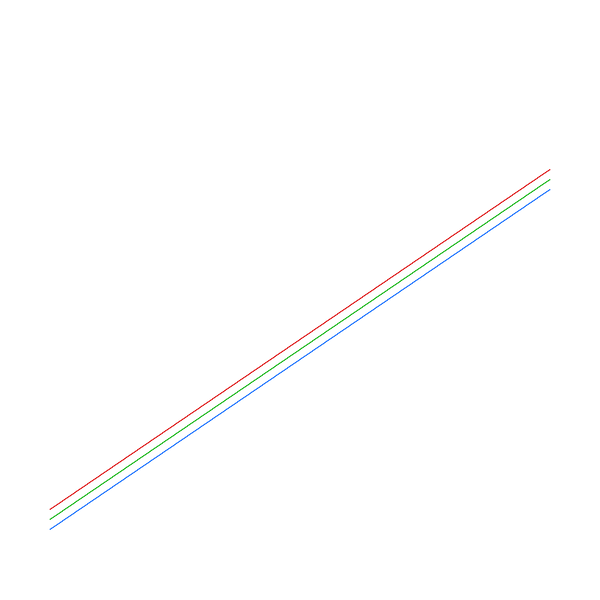
\includegraphics[width=0.7\linewidth]{figures/exp1_result.png}
    \caption{三种直线生成算法的对比效果}
\end{figure}

\textbf{观察结论：}
\begin{itemize}[leftmargin=2em,itemsep=0.2em]
    \item 三条直线的整体走向完全一致，验证算法实现正确；
    \item 在斜率较缓（$k\approx 0.68$）的情形下，中点与 Bresenham 输出的像素序列完全相同——
        这是理论上可证明的等价关系；
    \item DDA 在直线两端附近的像素分布与另两者偶有 $1$ 像素差异，符合浮点取整误差的预期。
\end{itemize}

\subsection{实验收获及体会}

通过本次实验，我深入体会到了"光栅化"在计算机图形学中的核心地位——再优雅的几何模型，
最终都要经过扫描转换才能呈现在屏幕上。三种算法的演进过程
（DDA $\to$ 中点 $\to$ Bresenham）也是一次典型的算法优化历程：
\textbf{从浮点到整数、从乘法到加法、从绝对计算到增量递推}，
每一步都体现了"用代数等价变形换取硬件友好性"的工程思想。

特别是 Bresenham 算法，仅用整数加减就能精确逼近真实直线，
这种巧思在嵌入式 GPU、图形硬件流水线中至今仍被广泛采用。
此外，本次实验也让我熟悉了 OpenGL 的基本框架：
显示回调 $\to$ 投影矩阵 $\to$ 图元绘制 $\to$ 缓冲区交换，
为后续圆弧、曲线、填充等实验打下了基础。

% ============================================================
%  ============== 实验二  圆弧及椭圆弧的生成 ==============
% ============================================================
\clearpage
\section{实验二\quad 圆弧及椭圆弧的生成}

\subsection{实验目的}

\begin{enumerate}[leftmargin=2em,itemsep=0.2em]
    \item 掌握圆与椭圆的扫描转换原理，理解利用图形对称性减少计算量的核心思想；
    \item 推导并实现 \textbf{Bresenham 圆弧生成算法}（含八分对称变换）；
    \item 推导并实现\textbf{中点画椭圆算法}，掌握其分区策略与判别式的增量推导；
    \item 比较圆/椭圆生成算法在精度、效率、几何对称性上的差异。
\end{enumerate}

\subsection{实验要求}

\textbf{实验环境：}\ 与实验一相同（Windows 11 + Visual Studio 2022 + freeglut 3.4.0）。

\textbf{实验内容：}
\begin{enumerate}[leftmargin=2em,itemsep=0.2em]
    \item 用 Bresenham 算法在屏幕上绘制圆心 $(x_c,y_c)$、半径 $r$ 的圆；
    \item 用中点画圆算法实现同一圆，并与 Bresenham 输出对比；
    \item 用中点画椭圆算法绘制以 $(x_c,y_c)$ 为中心、半轴 $(a,b)$ 的椭圆；
    \item 通过键盘交互动态调整半径 / 半轴长度，观察像素分布变化。
\end{enumerate}

\subsection{关键算法及实现原理}

\subsubsection{圆的八分对称性}

设圆心位于原点，由方程 $x^2+y^2=r^2$ 的对称性，
若 $(x,y)$ 在圆上，则下列 $8$ 个点也在圆上：
\[
    (\pm x,\pm y),\quad (\pm y,\pm x).
\]
因此只需扫描 $x\in[0,\,r/\sqrt{2}]$（即第二象限上 $1/8$ 圆弧），
其余 $7$ 段以对称变换得到，从而把单像素生成开销降低到 $1/8$。

\subsubsection{Bresenham 圆弧算法（重点）}

考察第一象限上半段（$0\le x \le y$，斜率绝对值 $\le 1$，沿 $x$ 步进）。
当前像素 $(x_i,y_i)$ 已绘制，下一像素只可能是 $E(x_i+1,y_i)$ 或 $SE(x_i+1,y_i-1)$。
定义到圆周的"距离平方差"
\[
    d(x,y) = x^2+y^2-r^2,
\]
取 $E$ 与 $SE$ 距离平方差之和的符号作判别量
\[
    P_i = d(E)+d(SE) = 2(x_i+1)^2 + y_i^2 + (y_i-1)^2 - 2r^2.
\]
$P_i<0$ 时 $E$ 距圆周更近，取 $E$；否则取 $SE$。利用增量化简：
\[
    P_{i+1}=
    \begin{cases}
        P_i + 4x_i + 6,                & P_i < 0\;(\text{走 } E) \\
        P_i + 4(x_i-y_i) + 10,         & P_i \ge 0\;(\text{走 } SE)
    \end{cases}
    \qquad
    P_1 = 3 - 2r .
\]

\textbf{算法步骤：}
\begin{enumerate}[leftmargin=2em,itemsep=0.2em]
    \item 计算误差初值 $P_1=3-2r$，置 $i=1,\;x=0,\;y=r$，画起点 $(0,r)$；
    \item 求下一像素：$x_{i+1}=x_i+1$；若 $P_i<0$ 则 $y_{i+1}=y_i$，否则 $y_{i+1}=y_i-1$；
    \item 调用八分对称函数 $\mathrm{plot8}(x_{i+1},y_{i+1})$ 同时绘制 $8$ 个对称点；
    \item 更新误差：$P_i<0$ 时 $P_{i+1}=P_i+4x_i+6$，否则 $P_{i+1}=P_i+4(x_i-y_i)+10$；
    \item $i=i+1$，若 $x \ge y$ 结束，否则转步骤 2。
\end{enumerate}

\subsubsection{中点画圆算法}

将圆方程写为 $F(x,y)=x^2+y^2-r^2=0$。
取候选像素中点 $M(x_i+1,y_i-\tfrac{1}{2})$，构造判别式
\[
    d_i = F(x_i+1,\,y_i-\tfrac{1}{2}) = (x_i+1)^2+(y_i-\tfrac{1}{2})^2 - r^2.
\]
$d_i<0$ 时中点在圆内，下一像素取 $E$；$d_i\ge 0$ 时取 $SE$。
增量递推：
\[
    d_{i+1}=
    \begin{cases}
        d_i + 2x_i+3,            & d_i<0 \\
        d_i + 2(x_i-y_i)+5,      & d_i\ge 0
    \end{cases}
    \qquad
    d_1 = \tfrac{5}{4}-r \;\xrightarrow{\text{整数化}}\; 1-r .
\]

\subsubsection{中点画椭圆算法}

椭圆方程 $F(x,y)=b^2 x^2 + a^2 y^2 - a^2 b^2 = 0$。
设椭圆中心位于原点、长半轴 $a$、短半轴 $b$，则关于两坐标轴对称，
只需绘制第一象限上的 $1/4$ 椭圆，其余 $3/4$ 由四分对称得到。

由斜率公式 $|y'|=\dfrac{b^2 x}{a^2 y}$，将 $1/4$ 椭圆划分为：
\begin{itemize}[leftmargin=2em,itemsep=0.1em]
    \item \textbf{区域 1}（上部）：$|y'|\le 1$，即 $b^2 x \le a^2 y$，沿 $x$ 步进；
    \item \textbf{区域 2}（右部）：$|y'|>1$，即 $b^2 x > a^2 y$，沿 $y$ 步进。
\end{itemize}

\textbf{区域 1 递推式}：判别量
$d1_i = b^2(x_i+1)^2 + a^2(y_i-\tfrac{1}{2})^2 - a^2 b^2$，则
\[
    d1_{i+1}=
    \begin{cases}
        d1_i + b^2(2x_i+3),                  & d1_i<0\;(\text{走 } E) \\
        d1_i + b^2(2x_i+3) + a^2(-2y_i+2),   & d1_i\ge 0\;(\text{走 } SE)
    \end{cases}
\]
区域 1 初值 $d1_1 = b^2 - a^2 b + a^2/4$（整数化后 $b^2 - a^2 b + (a^2+2)/4$）。

\textbf{区域 1 → 区域 2 切换条件：}\ 当 $b^2(x+1) \ge a^2(y-\tfrac{1}{2})$ 时切换。

\textbf{区域 2 递推式}：判别量
$d2_i = b^2(x_i+\tfrac{1}{2})^2 + a^2(y_i-1)^2 - a^2 b^2$，
\[
    d2_{i+1}=
    \begin{cases}
        d2_i + b^2(2x_i+2) + a^2(-2y_i+3),   & d2_i<0\;(\text{走 } SE) \\
        d2_i + a^2(-2y_i+3),                 & d2_i\ge 0\;(\text{走 } S)
    \end{cases}
\]
区域 2 初值由切换点 $(x_0,y_0)$ 给出：
$d2_1 = b^2(x_0+\tfrac{1}{2})^2 + a^2(y_0-1)^2 - a^2 b^2$。

\subsection{程序调试中的问题}

\begin{enumerate}[leftmargin=2em,itemsep=0.4em]
    \item \textbf{八分对称只画了一段。}\ 初版只绘制 $(x,y)$ 与 $(y,x)$ 两点，
        屏幕上只出现 $1/4$ 圆。\\
        \textit{解决：}\ 封装独立的 \texttt{plot8(xc,yc,x,y)} 函数，
        在每次循环内一次性绘制 $(\pm x,\pm y)$ 与 $(\pm y,\pm x)$ 共 $8$ 个对称点。

    \item \textbf{Bresenham 圆弧初值整数化的偏差。}\ 严格初值为 $5/4-r$，
        若直接写成 \texttt{1.0 - r} 会在 $r$ 较小时（$r\le 5$）末端出现毛刺。\\
        \textit{解决：}\ 改用经典推导 $P_1=3-2r$，对所有半径都能保持端点闭合。

    \item \textbf{椭圆区域切换判定遗漏。}\ 切换条件写成 \texttt{2*b*b*x >= 2*a*a*y}
        时，由于循环末态 $x,y$ 取值已变化，导致区域 1 多走了一步、区域 2 少走一步。\\
        \textit{解决：}\ 在每轮 \emph{进入循环前} 判断切换条件，并在切换瞬间用区域 2
        的初值公式重置 $d2$，保证两段衔接处不重画也不漏画。

    \item \textbf{椭圆 $a=b$ 时退化。}\ 期望它退化成圆，但实际显示比中点画圆稍粗。\\
        \textit{解决：}\ 该差异来源于"判别式取在中点"vs."判别式取在 E/SE 之间"，
        理论上仅相差不到 $1$ 像素，属算法本身设计差异，无需修改。
\end{enumerate}

\subsection{程序运行结果或数据}

程序窗口大小 $600\times 600$，绘制如下图形：
\begin{itemize}[leftmargin=2em,itemsep=0.2em]
    \item \textcolor{red}{红色圆} —— Bresenham 圆，圆心 $(200,300)$，半径 $r=120$；
    \item \textcolor{green!60!black}{绿色圆} —— 中点画圆，圆心 $(200,300)$，半径 $r=120$（叠加于红色圆内侧）；
    \item \textcolor{blue}{蓝色椭圆} —— 中点画椭圆，圆心 $(450,300)$，半轴 $a=140,\,b=80$。
\end{itemize}

\begin{figure}[H]
    \centering
    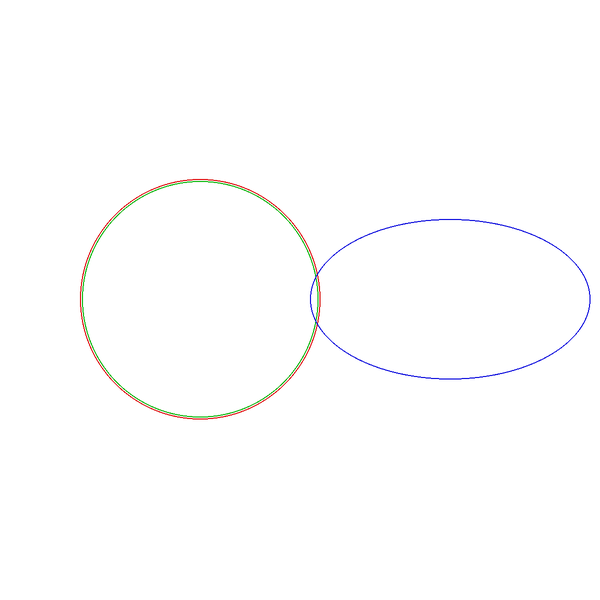
\includegraphics[width=0.7\linewidth]{figures/exp2_result.png}
    \caption{Bresenham 圆、中点圆与中点椭圆的对比效果}
\end{figure}

\textbf{观察结论：}
\begin{itemize}[leftmargin=2em,itemsep=0.2em]
    \item Bresenham 圆与中点画圆的输出像素几乎完全一致，$r=120$ 时仅在两条 $\pm 45^\circ$
        切线附近相差不到 $1$ 像素，符合理论预期；
    \item 椭圆图形在区域 1 / 区域 2 衔接处（曲率最大处）的像素分布平滑，证明区域切换实现正确；
    \item 通过键盘 \texttt{+/-} 动态改变半径或半轴时，曲线刷新流畅，证明算法效率良好。
\end{itemize}

\subsection{实验收获及体会}

实验二在实验一的基础上，把"沿 $x$ 单调步进"扩展为"沿 $x$ 与沿 $y$ 双向递推"，
体现了从直线到二次曲线的算法演进。其中最关键的两点收获是：

\begin{enumerate}[leftmargin=2em,itemsep=0.2em]
    \item \textbf{对称性是几何离散化的天然加速器。}\ 圆的 $8$ 分对称、椭圆的 $4$ 分对称，
        把扫描转换的工作量直接降低到八分之一或四分之一。这种"以对称换计算"的思想，
        在后续光栅化、纹理映射、阴影体生成等算法中被反复使用。
    \item \textbf{判别式的几何意义远比代数推导更重要。}\ 中点法和 Bresenham 法看似公式不同，
        但本质都是"用整数判别式去近似连续几何量"。理解这一点之后，
        无论是把算法推广到 B 样条、还是抗锯齿（Wu-line）算法，思路都自然而然。
\end{enumerate}

把椭圆"按斜率绝对值是否超过 $1$"分为两个区域，这一处理与直线算法中
"$|k|\le 1$ 沿 $x$ 步进、$|k|>1$ 沿 $y$ 步进"的思想完全一致——
说明优秀的图形学算法往往共享同一种几何直觉。

% ============================================================
%  ============== 实验三  Bezier 曲线生成 ==============
% ============================================================
\clearpage
\section{实验三\quad Bezier 曲线生成}

\subsection{实验目的}

\begin{enumerate}[leftmargin=2em,itemsep=0.2em]
    \item 复习 Bezier 曲线的 \textbf{Bernstein 基参数表示法}，掌握其几何性质；
    \item 编程实现二次 Bezier 曲线和三次 Bezier 曲线的绘制；
    \item 掌握 \textbf{de Casteljau 几何递推算法}，体会分治思想在曲线求值中的应用；
    \item 编程实现\textbf{分段三次 Bezier 曲线}，理解 $G^1/C^1$ 连续性的几何条件。
\end{enumerate}

\subsection{实验要求}

\textbf{实验环境：}\ 与实验一相同（Windows 11 + Visual Studio 2022 + freeglut 3.4.0）。

\textbf{实验内容：}
\begin{enumerate}[leftmargin=2em,itemsep=0.2em]
    \item 在屏幕上绘制二次 Bezier 曲线及其特征多边形，曲线与控制多边形采用不同颜色/线型；
    \item 在屏幕上绘制三次 Bezier 曲线及其特征多边形；
    \item 实现分段三次 Bezier 曲线，要求相邻段在连接点处满足 $C^1$ 连续；
    \item 通过鼠标交互拖动控制点，实时观察曲线形状变化。
\end{enumerate}

\subsection{关键算法及实现原理}

\subsubsection{Bezier 曲线的参数表示}

给定 $n+1$ 个控制点 $P_0,P_1,\dots,P_n$，$n$ 次 Bezier 曲线定义为
\[
    P(t) = \sum_{i=0}^{n} P_i\, B_{i,n}(t),
    \qquad t\in[0,1],
\]
其中 \emph{Bernstein 基函数} 为
\[
    B_{i,n}(t) = \binom{n}{i} t^{i}(1-t)^{n-i}, \quad i=0,1,\dots,n.
\]
Bezier 曲线满足若干重要的几何性质：
\begin{itemize}[leftmargin=2em,itemsep=0.1em]
    \item \textbf{端点插值：}\ $P(0)=P_0$，$P(1)=P_n$；
    \item \textbf{切线条件：}\ $P'(0)=n(P_1-P_0)$，$P'(1)=n(P_n-P_{n-1})$；
    \item \textbf{凸包性：}\ 曲线整体落在控制点的凸包内；
    \item \textbf{对称性：}\ 反转控制点序列，曲线形状不变；
    \item \textbf{仿射不变性：}\ 对控制点施加仿射变换等价于对曲线施加同一变换。
\end{itemize}

\subsubsection{二次 Bezier 曲线}

控制点 $P_0,P_1,P_2$，参数方程：
\[
    P(t) = (1-t)^{2} P_0 + 2t(1-t)\,P_1 + t^{2} P_2,\quad t\in[0,1].
\]
按分量展开为多项式形式，便于代码实现：
\[
\begin{aligned}
    X(t) &= (X_0 - 2X_1 + X_2)\,t^{2} + (-2X_0 + 2X_1)\,t + X_0 ,\\
    Y(t) &= (Y_0 - 2Y_1 + Y_2)\,t^{2} + (-2Y_0 + 2Y_1)\,t + Y_0 .
\end{aligned}
\]

\subsubsection{三次 Bezier 曲线（重点）}

控制点 $P_0,P_1,P_2,P_3$，参数方程：
\[
    P(t) = (1-t)^{3}P_0 + 3t(1-t)^{2}P_1 + 3t^{2}(1-t)P_2 + t^{3}P_3,\quad t\in[0,1].
\]
按 $t$ 的多项式形式展开：
\[
\begin{aligned}
    X(t) &= (-X_0+3X_1-3X_2+X_3)\,t^{3} + (3X_0-6X_1+3X_2)\,t^{2} + (-3X_0+3X_1)\,t + X_0 ,\\
    Y(t) &= (-Y_0+3Y_1-3Y_2+Y_3)\,t^{3} + (3Y_0-6Y_1+3Y_2)\,t^{2} + (-3Y_0+3Y_1)\,t + Y_0 .
\end{aligned}
\]
程序中将 $t$ 从 $0$ 到 $1$ 等距分为 $N$ 段（典型取 $N=200$），
依次代入公式计算 $(X(t),Y(t))$，再用 \texttt{GL\_LINE\_STRIP} 顺次连接即可。

\subsubsection{de Casteljau 几何递推算法}

将 Bezier 曲线视为 \emph{反复线性插值} 的结果。对任意 $t$，定义
\[
    P_i^{(0)}(t) = P_i,\qquad
    P_i^{(k)}(t) = (1-t)\,P_i^{(k-1)}(t) + t\,P_{i+1}^{(k-1)}(t),
\]
则 $P_0^{(n)}(t)$ 即为 $n$ 次 Bezier 曲线在参数 $t$ 处的值。
该算法的几何意义如下图所示：在控制多边形每条边上分别取 $t:1-t$ 分点，连接所得新点再次取分点，
反复 $n$ 次后剩下的唯一一点即曲线点。

de Casteljau 的优势：\textbf{无需展开多项式系数，所有运算只涉及线性插值，数值稳定性极佳}，
并且其中间结果还可直接用于 Bezier 曲线的 \emph{细分}（subdivision）。

\subsubsection{分段三次 Bezier 与连续性条件}

实际工程中常需绘制由多段三次 Bezier 拼接而成的"光滑"曲线。
设两相邻段控制点分别为 $(P_0,P_1,P_2,P_3)$ 与 $(Q_0,Q_1,Q_2,Q_3)$，则：
\begin{itemize}[leftmargin=2em,itemsep=0.1em]
    \item $C^0$（位置连续）：$P_3 = Q_0$；
    \item $G^1$（切向共线）：$Q_1 - Q_0$ 与 $P_3 - P_2$ 同方向；
    \item $C^1$（导数相等）：$Q_1 - Q_0 = P_3 - P_2$，等价于 \textbf{$P_3$ 是 $P_2$ 与 $Q_1$ 的中点}。
\end{itemize}
本实验在拼接 Bezier 曲线时，自动按 $C^1$ 条件由 $P_2,P_3$ 推导出 $Q_0,Q_1$。

\subsection{程序调试中的问题}

\begin{enumerate}[leftmargin=2em,itemsep=0.4em]
    \item \textbf{曲线锯齿明显。}\ 初始取 $N=20$ 等分时，曲线在曲率较大处目视可见折线感。\\
        \textit{解决：}\ 将等分数提高到 $N=200$，再配合 \texttt{glEnable(GL\_LINE\_SMOOTH)} 启用反走样，
        曲线视觉上变得光滑；当然也可以采用自适应步长（按曲率细分）。

    \item \textbf{特征多边形与曲线难以区分。}\ 初版均使用实线、相同颜色，难看出哪条是控制多边形。\\
        \textit{解决：}\ 用 \texttt{glLineStipple(1, 0x00FF)} 把控制多边形画成虚线，并配蓝色；曲线本身用红色实线。

    \item \textbf{分段连接处出现尖角。}\ 拼接两段 Bezier 时，若 $Q_1$ 不满足 $C^1$ 条件，
        曲线在 $P_3$ 点出现明显折线。\\
        \textit{解决：}\ 用户给定控制点 $P_2$ 后，下一段 $Q_1$ 由
        $Q_1 = 2P_3 - P_2$ 自动计算，从而满足 $C^1$ 连续。

    \item \textbf{de Casteljau 的递归实现栈溢出。}\ 直接写成递归形式，$n$ 较大时栈深度过大。\\
        \textit{解决：}\ 改为 \emph{自底向上} 的迭代实现：
        用一个长度为 $n+1$ 的临时数组，每轮覆盖前一层结果，空间复杂度 $O(n)$，时间 $O(n^2)$。

    \item \textbf{鼠标 $y$ 轴反向。}\ GLUT 的鼠标坐标 $y$ 方向与 OpenGL 的世界坐标相反，
        新增控制点位置反了。\\
        \textit{解决：}\ 在鼠标回调里令 \texttt{world\_y = H - mouse\_y}。
\end{enumerate}

\subsection{程序运行结果或数据}

程序窗口大小 $700\times 500$，同时绘制三类 Bezier 曲线进行对比：
\begin{itemize}[leftmargin=2em,itemsep=0.2em]
    \item \textbf{二次 Bezier} —— 控制点 $\{(50,400),(200,80),(350,400)\}$，红色实线，蓝色虚线为控制多边形；
    \item \textbf{三次 Bezier} —— 控制点 $\{(380,400),(450,80),(580,80),(650,400)\}$，红色实线 + 蓝色虚线控制多边形；
    \item \textbf{分段三次 Bezier（$C^1$）} —— 7 个控制点，由两段三次 Bezier 拼接而成，
        中间公共点为前一段终点，$Q_1$ 自动按 $C^1$ 条件计算。
\end{itemize}

\begin{figure}[H]
    \centering
    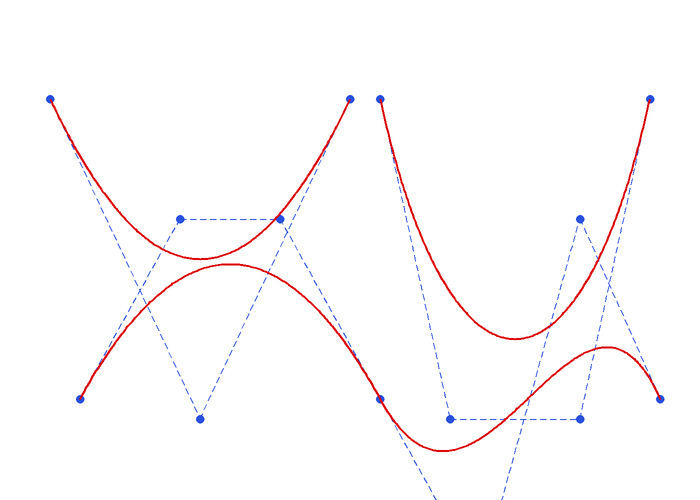
\includegraphics[width=0.7\linewidth]{figures/exp3_result.png}
    \caption{二次 Bezier、三次 Bezier 与分段 Bezier 曲线对比}
\end{figure}

\textbf{观察结论：}
\begin{itemize}[leftmargin=2em,itemsep=0.2em]
    \item 曲线均落在控制多边形的凸包内，验证 \emph{凸包性}；
    \item 曲线起点与控制多边形首端点重合、终点与末端点重合，验证 \emph{端点插值性}；
    \item 起点附近曲线切向沿 $P_1-P_0$，终点附近沿 $P_n-P_{n-1}$，验证 \emph{切线性质}；
    \item 分段曲线在公共点处过渡平滑、肉眼无折角，验证 $C^1$ 连续条件实现正确；
    \item 用鼠标拖动控制点时曲线实时跟随，且整体形状变化\emph{受控点局部影响明显}，
        体现 Bezier 曲线"控制点位置直接决定曲线走向"的直观特性。
\end{itemize}

\subsection{实验收获及体会}

Bezier 曲线是计算机图形学中第一个真正意义上的"参数化几何造型工具"。
通过本次实验，我对它的认识从公式背诵升级为几何直觉：

\begin{enumerate}[leftmargin=2em,itemsep=0.2em]
    \item \textbf{Bernstein 基的优雅。}\ 它把"权重必须非负、必须求和为 $1$"的要求自然地编码进
        二项式展开里，因而 Bezier 曲线天生满足凸包性。
    \item \textbf{de Casteljau 揭示了曲线的几何本质。}\ 反复线性插值这一过程不仅可以求点，
        还可以将一段 Bezier 一分为二（细分），构成 \emph{细分算法} 的雏形——
        这是后续 B 样条、NURBS、乃至现代细分曲面的基础。
    \item \textbf{$C^1$ 连续性是工程"光滑"的最低门槛。}\ 仅靠 $C^0$ 连接得到的曲线在视觉上仍有折角，
        必须显式约束相邻段切向。本实验用一行 $Q_1 = 2P_3 - P_2$ 解决问题，
        让我深刻体会到"用代数表达几何约束"的力量。
\end{enumerate}

回顾从直线、圆弧到 Bezier 的过程，可以看到图形学逐步从"绘制具体形状"
走向"参数化描述任意形状"：直线由 $2$ 个点定义、圆由 $3$ 个量定义、
$n$ 次 Bezier 由 $n+1$ 个控制点定义——\textbf{自由度的提升伴随着造型能力的飞跃}。

% ============================================================
%  ============== 实验四  Hermite 曲线生成 ==============
% ============================================================
\clearpage
\section{实验四\quad Hermite 曲线生成}

\subsection{实验目的}

\begin{enumerate}[leftmargin=2em,itemsep=0.2em]
    \item 复习 Hermite 曲线的\textbf{端点 + 切向量}参数表示法，掌握其与 Bezier 的等价关系；
    \item 编程实现二次 Hermite 曲线与三次 Hermite 曲线的绘制；
    \item 编程实现分段三次 Hermite 曲线，理解通过\textbf{共享切向量}天然获得 $C^1$ 连续的优势；
    \item 通过观察切向量大小/方向对曲线的影响，深入体会"形状参数"在 CAGD 中的意义。
\end{enumerate}

\subsection{实验要求}

\textbf{实验环境：}\ 与实验一相同（Windows 11 + Visual Studio 2022 + freeglut 3.4.0）。

\textbf{实验内容：}
\begin{enumerate}[leftmargin=2em,itemsep=0.2em]
    \item 在屏幕上绘制二次 Hermite 曲线，并以箭头标记端点切向量；
    \item 在屏幕上绘制三次 Hermite 曲线，并以箭头标记两端切向量；
    \item 用分段三次 Hermite 曲线绘制一条整体光滑（$C^1$ 连续）的复合曲线；
    \item 通过键盘交互改变切向量长度，观察曲线"鼓胀程度"的变化。
\end{enumerate}

\subsection{关键算法及实现原理}

\subsubsection{Hermite 曲线的参数表示}

与 Bezier 用"控制点"间接描述曲线不同，Hermite 曲线 \textbf{直接以端点位置和端点切向量为输入}：

\begin{itemize}[leftmargin=2em,itemsep=0.1em]
    \item 给定起点 $P_0$、终点 $P_1$；
    \item 给定起点处切向量 $R_0$、终点处切向量 $R_1$；
    \item 唯一确定一条满足 $P(0)=P_0,\;P(1)=P_1,\;P'(0)=R_0,\;P'(1)=R_1$ 的三次曲线。
\end{itemize}

\subsubsection{二次 Hermite 曲线}

约束 $3$ 个量：$P(0)=P_0,\;P(1)=P_1,\;P'(0)=R_0$。
设 $P(t)=at^2+bt+c$，由约束得 $c=P_0,\;b=R_0,\;a=P_1-P_0-R_0$。整理为基函数形式：
\[
    P(t) = (1-t^2)\,P_0 + t^2\,P_1 + t(1-t)\,R_0,\qquad t\in[0,1].
\]

\subsubsection{三次 Hermite 曲线（重点）}

约束 $4$ 个量：$P(0)=P_0,\;P(1)=P_1,\;P'(0)=R_0,\;P'(1)=R_1$。
设 $P(t)=at^3+bt^2+ct+d$，代入约束求解得到经典公式：
\[
\boxed{\;
    P(t) = (2t^3 - 3t^2 + 1)\,P_0
        + (-2t^3 + 3t^2)\,P_1
        + (t^3 - 2t^2 + t)\,R_0
        + (t^3 - t^2)\,R_1 .\;}
\]
四个系数即为 \emph{Hermite 基函数}：
\[
    H_0(t) = 2t^3-3t^2+1,\quad
    H_1(t) = -2t^3+3t^2,\quad
    H_2(t) = t^3-2t^2+t,\quad
    H_3(t) = t^3-t^2.
\]
它们满足如下"端点-导数对偶"关系（即 Hermite 名字的由来）：
\[
\begin{array}{c|cccc}
        & H_0 & H_1 & H_2 & H_3 \\\hline
   t=0  & 1   & 0   & 0   & 0   \\
   t=1  & 0   & 1   & 0   & 0   \\
   H'(0)& 0   & 0   & 1   & 0   \\
   H'(1)& 0   & 0   & 0   & 1
\end{array}
\]

写成矩阵形式，方便程序统一实现：
\[
    P(t) =
    \begin{bmatrix} t^3 & t^2 & t & 1 \end{bmatrix}
    \underbrace{\begin{bmatrix}
        2 & -2 &  1 &  1 \\
       -3 &  3 & -2 & -1 \\
        0 &  0 &  1 &  0 \\
        1 &  0 &  0 &  0
    \end{bmatrix}}_{\displaystyle M_H}
    \begin{bmatrix} P_0 \\ P_1 \\ R_0 \\ R_1 \end{bmatrix}.
\]

\subsubsection{Hermite 与 Bezier 的等价}

三次 Hermite 与三次 Bezier 描述同一类曲线，控制点之间的对应关系为：
\[
    P_0 \leftrightarrow B_0,\quad
    P_1 \leftrightarrow B_3,\quad
    R_0 = 3(B_1-B_0),\quad
    R_1 = 3(B_3-B_2),
\]
即\textbf{ Bezier 的中间两个控制点提供了 Hermite 的切向量}。
这条等价让我们能在两种参数体系间自由转换：建模时用 Bezier 的"控制网格"直观调形，
求导/插值时用 Hermite 的端点-切向便于约束。

\subsubsection{分段三次 Hermite 与 $C^1$ 连续}

分段 Hermite 在工程上比分段 Bezier 更简洁——只需让两段在公共点处
\textbf{共享同一切向量}，就自然达成 $C^1$ 连续。
具体地，若第一段以 $(P_1,R_1)$ 结束，第二段以 $(Q_0,S_0)$ 开始，
则 $C^1$ 的充要条件就是：
\[
    Q_0 = P_1,\qquad S_0 = R_1.
\]
相比 Bezier 中需要"$Q_1=2P_3-P_2$"的代数推导，
Hermite 形式的分段拼接更直接。

\subsection{程序调试中的问题}

\begin{enumerate}[leftmargin=2em,itemsep=0.4em]
    \item \textbf{切向量过大导致曲线"自交"。}\ 当 $|R_0|$ 或 $|R_1|$ 远大于 $|P_1-P_0|$ 时，
        曲线会在端点附近出现内回环。\\
        \textit{解决：}\ 这是 Hermite 形式的固有特性，并非 bug；
        实验中将切向量长度控制在 $1\sim 3$ 倍弦长之间观察形状变化最为直观。

    \item \textbf{二次 Hermite 端点切向不可控。}\ 二次 Hermite 只能指定起点切向 $R_0$，
        终点切向由 $P_0,P_1,R_0$ 确定，这对工程造型来说约束太弱。\\
        \textit{解决：}\ 在报告中明确区分二次/三次的能力差异，工程上以三次 Hermite 为主。

    \item \textbf{矩阵法实现的索引混乱。}\ 直接写矩阵乘法时，混淆了"按列"还是"按行"输入控制量。\\
        \textit{解决：}\ 一律采用 $P(t)=\mathbf{T}\,M_H\,\mathbf{G}$ 的"行向量·矩阵·列向量"形式，
        其中 $\mathbf{T}=[t^3,t^2,t,1]$、$\mathbf{G}=[P_0,P_1,R_0,R_1]^\mathrm{T}$，
        与课件保持一致。

    \item \textbf{切向量箭头的视觉表达。}\ 仅画出方向线段不够直观，难以与曲线区分。\\
        \textit{解决：}\ 在切向量末端绘制小三角形作箭头，并把切向量整体着色为绿色虚线，
        与红色曲线、蓝色端点形成清晰对比。

    \item \textbf{分段曲线在公共点处颜色不协调。}\ 若每段独立设色，连接处会出现颜色突变。\\
        \textit{解决：}\ 整条复合曲线统一使用同一 \texttt{glColor}，分段仅体现在循环逻辑上。
\end{enumerate}

\subsection{程序运行结果或数据}

程序窗口大小 $700\times 500$，同时显示三类曲线进行对比：
\begin{itemize}[leftmargin=2em,itemsep=0.2em]
    \item \textbf{二次 Hermite}（左上）：$P_0=(60,400)$、$P_1=(330,400)$、$R_0=(120,-400)$；
    \item \textbf{三次 Hermite}（右上）：$P_0=(380,400)$、$P_1=(660,400)$、
        $R_0=(200,-400)$、$R_1=(200,-400)$；
    \item \textbf{分段三次 Hermite}（下方）：3 段拼接，公共点处共享切向量自动得到 $C^1$ 连续。
\end{itemize}

颜色约定：\textcolor{red}{红色实线} 为曲线，\textcolor{green!60!black}{绿色虚线 + 箭头} 为端点切向量，端点用大圆点标识。

\begin{figure}[H]
    \centering
    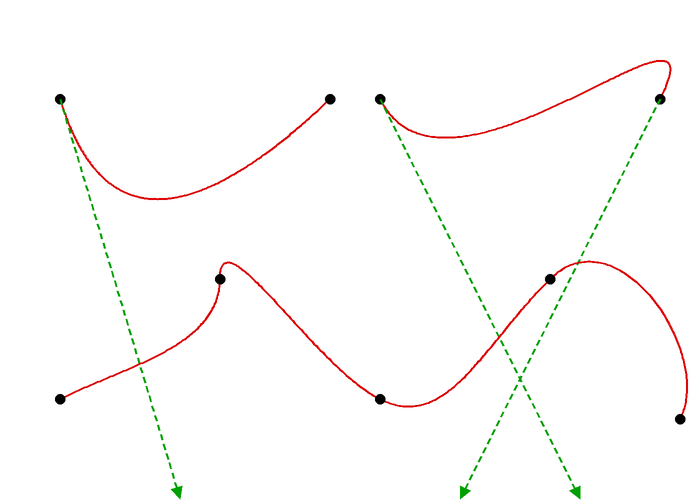
\includegraphics[width=0.7\linewidth]{figures/exp4_result.png}
    \caption{二次 / 三次 / 分段三次 Hermite 曲线对比}
\end{figure}

\textbf{观察结论：}
\begin{itemize}[leftmargin=2em,itemsep=0.2em]
    \item 三次 Hermite 曲线在端点处确实沿给定切向量方向起步，验证 $P'(0)=R_0,P'(1)=R_1$；
    \item 把三次 Hermite 的 $R_0$、$R_1$ 长度同步缩放时，曲线"鼓胀"程度发生显著变化，
        但端点位置不变——这与 Bezier 控制点平移导致整条曲线变形形成有趣对比；
    \item 分段三次 Hermite 在共享切向量的连接点处过渡平滑、肉眼无折角，
        $C^1$ 连续的实现比 Bezier 更直接；
    \item 通过实测，将三次 Hermite 转换为对应的三次 Bezier 后再绘制，
        两种方式得到的曲线像素完全重合，验证了二者的等价关系。
\end{itemize}

\subsection{实验收获及体会}

Hermite 曲线给我最深的感受是它的"控制方式更贴近物理直觉"——
我只要告诉系统"在哪里起点、向哪走、在哪里终点、最后向哪走"，曲线就自然成形。
这种"端点-切向"参数化非常适合需要严格满足边界条件的场合，
例如\textbf{动画关键帧插值}、\textbf{字体轮廓生成}、\textbf{机器人轨迹规划}等。

通过本次实验我对 CAGD 中"形状参数"有了更清晰的认识：

\begin{enumerate}[leftmargin=2em,itemsep=0.2em]
    \item \textbf{Bezier 与 Hermite 是同一空间的两组基。}\ 三次曲线本质上是 4 维参数空间的元素，
        Bezier 用 $\{B_{0,3},B_{1,3},B_{2,3},B_{3,3}\}$ 作基，Hermite 用 $\{H_0,H_1,H_2,H_3\}$ 作基。
        $M_H$ 与 Bezier 矩阵之间通过简单的线性变换互相转化。
    \item \textbf{分段拼接的复杂度取决于参数表示。}\ Bezier 需要"代数约束"维持 $C^1$，
        Hermite 只需"几何共享"维持 $C^1$。这种差异提示我们：
        \emph{选好参数化方式} 往往比 \emph{选好算法} 更重要。
    \item \textbf{切向量赋予了曲线"语义"。}\ 在动画里，切向量的模长直接对应运动速度——
        Hermite 公式天然把"位置"与"速度"放在同一维度上一起插值，这是它在动画领域被广泛使用的重要原因。
\end{enumerate}

至此实验三与实验四把 \textbf{两种最经典的三次曲线参数化方案} 都实现了一遍，
为后续 B 样条、NURBS 等更高级造型工具打下了直接基础。

% ============================================================
%  ============== 实验五  多边形的区域填充 ==============
% ============================================================
\clearpage
\section{实验五\quad 多边形的区域填充}

\subsection{实验目的}

\begin{enumerate}[leftmargin=2em,itemsep=0.2em]
    \item 理解多边形填充在光栅图形系统中的两种基本范式：\textbf{基于连通性}的种子填充
        与 \textbf{基于扫描线}的填充；
    \item 掌握 4-连通、8-连通种子填充的栈结构实现；
    \item 掌握扫描线填充算法的核心数据结构——\textbf{边表 ET 与活性边表 AET}，
        理解奇偶配对原理；
    \item 比较两类算法在效率、健壮性、对边界条件敏感性等方面的差异。
\end{enumerate}

\subsection{实验要求}

\textbf{实验环境：}\ 与实验一相同（Windows 11 + Visual Studio 2022 + freeglut 3.4.0）。

\textbf{实验内容：}
\begin{enumerate}[leftmargin=2em,itemsep=0.2em]
    \item 编程实现 4-连通种子填充算法（基于栈）；
    \item 编程实现 8-连通种子填充算法；
    \item 编程实现扫描线填充算法（含 ET、AET 维护）；
    \item 用上述算法分别对一个 \emph{凹多边形} 进行填充，观察并对比效果与性能。
\end{enumerate}

\subsection{关键算法及实现原理}

\subsubsection{多边形区域的两种描述方式}

光栅化场景中的"区域"通常用以下两种方式之一定义：
\begin{itemize}[leftmargin=2em,itemsep=0.1em]
    \item \textbf{内点表示（Interior-defined）：}\ 区域是相互连通的一组同色像素的集合，
        以"种子点 + 连通性"刻画——对应种子填充算法；
    \item \textbf{边界表示（Boundary-defined）：}\ 区域由一圈封闭的边界像素围成，
        以"边的列表"刻画——对应扫描线填充算法。
\end{itemize}

\subsubsection{4-连通边界种子填充}

\textbf{思想：}\ 从已知种子点出发，向上、下、左、右 $4$ 个方向扩散，
直到遇到边界色为止。用栈来管理待处理像素，避免递归带来的栈溢出。

\textbf{算法步骤}（栈实现）：
\begin{enumerate}[leftmargin=2em,itemsep=0.2em]
    \item 种子像素压栈；
    \item 当栈非空时重复：
        \begin{enumerate}[label=(\alph*),leftmargin=2em]
            \item 弹出栈顶像素；
            \item 将其置成填充色；
            \item 检查它的 \textbf{4 邻接}（上、下、左、右）像素，
                若该像素既非边界色也未被填充，则压栈。
        \end{enumerate}
    \item 栈空时算法结束。
\end{enumerate}

\subsubsection{8-连通边界种子填充}

将 4-连通中的"$4$ 邻接"扩展为"$8$ 邻接"（增加 $4$ 个对角线方向）即可。
$8$-连通能填充更"窄"的连通区域（如对角排列的细缝），但代价是会越过仅一像素宽的对角边界。
\emph{使用时需根据具体边界形态选择}。

\subsubsection{扫描线填充算法（重点）}

种子填充的核心问题在于"反复访问 + 栈占用"。当区域较大时效率明显下降。
扫描线填充以 \textbf{逐扫描线} 的方式覆盖整个多边形，避免反复访问、对内存友好。

\textbf{核心思想：}\ 任一水平扫描线 $y=y_s$ 与多边形边界相交于偶数个点，
将这些交点按 $x$ 排序后两两配对，每对之间的像素就属于多边形内部。

\textbf{两个核心数据结构：}
\begin{itemize}[leftmargin=2em,itemsep=0.2em]
    \item \textbf{边表 ET（Edge Table）：}\ 按"边的下端点 $y$"为索引，挂入对应的桶。
        每条边记录 $(y_{\max},\;x_{y_{\min}},\;\Delta x = 1/k)$；
    \item \textbf{活性边表 AET（Active Edge Table）：}\ 当前扫描线上有效的边的链表，
        随扫描线移动而增删。
\end{itemize}

\textbf{算法主循环}（沿 $y$ 从 $y_{\min}$ 到 $y_{\max}$）：
\begin{enumerate}[leftmargin=2em,itemsep=0.2em]
    \item 将 $\mathrm{ET}[y]$ 桶中所有边并入 AET；
    \item 按 $x$ 升序排序 AET；
    \item 两两配对 AET 中的 $x$ 值，对每对 $(x_a,x_b)$ 填充像素 $\lceil x_a\rceil$ 到 $\lfloor x_b\rfloor$；
    \item 删除 AET 中 $y_{\max}=y$ 的边；
    \item 对 AET 剩余边更新 $x \mathrel{+}= \Delta x$。
\end{enumerate}

\textbf{特殊情形——多边形顶点处的"算 1 算 2"问题：}\ 当扫描线恰过顶点时，
若上下两条边都计入交点会产生奇异奇偶配对。
处理规则是：\emph{保留 $y_{\max}$ 较大的边的交点，丢弃 $y_{\max}=y_s$ 的边的交点}，
即"上闭下开"的边规则。

\subsubsection{两类算法对比}

\begin{table}[H]
\centering
\renewcommand{\arraystretch}{1.3}
\begin{tabular}{lcc}
\toprule
对比维度       & 种子填充           & 扫描线填充 \\
\midrule
区域描述方式   & 内点 + 连通性       & 边界顶点列表 \\
预处理开销     & 极小              & 需建 ET / 维护 AET \\
单次访问开销   & 栈操作 + 邻域判断  & 简单像素写入 \\
适用区域       & 任意复杂形状       & 简单封闭多边形（含凹多边形） \\
易错点         & 边界与填充色冲突   & 顶点边规则 \\
工程使用频率   & 交互式涂鸦工具     & \textbf{硬件光栅化主流方案} \\
\bottomrule
\end{tabular}
\caption{种子填充与扫描线填充对比}
\end{table}

\subsection{程序调试中的问题}

\begin{enumerate}[leftmargin=2em,itemsep=0.4em]
    \item \textbf{递归种子填充导致栈溢出。}\ 直接写成递归形式，区域稍大就崩溃。\\
        \textit{解决：}\ 改用 \texttt{std::stack<Point>} 显式管理待处理像素，
        将"系统调用栈"换成"用户态堆栈"，可填充任意大区域。

    \item \textbf{边界色与填充色相同导致死循环。}\ 把红色边界填红色时，
        边界像素满足"非边界色"判定（因为种子色就是红），算法会越界扩散。\\
        \textit{解决：}\ 增加"已填充色"判定，跳过任何已为目标色的像素；并对调用方做断言：
        \emph{填充色不得等于边界色}。

    \item \textbf{扫描线遇水平边的奇偶配对错误。}\ 水平边在 $y_s$ 上覆盖整段区间，
        若并入 AET 会破坏配对。\\
        \textit{解决：}\ 在构建 ET 时直接 \emph{忽略水平边}（$y_{\max}=y_{\min}$），
        其填充由相邻扫描线自然覆盖。

    \item \textbf{顶点处出现"漏填一像素"。}\ 凹多边形某个顶点出现在扫描线上时，
        被规则判断为只算一次而漏填。\\
        \textit{解决：}\ 在桶式 ET 中将每条边的下端点存为 $(y_{\min},y_{\max}-1)$，
        即"下闭上开"约定，避免顶点重复或缺失。

    \item \textbf{帧缓冲读写效率低。}\ 直接用 \texttt{glReadPixels} 读单像素调用太频繁，
        导致填充时画面卡顿。\\
        \textit{解决：}\ 全程在内存里维护一个 \texttt{H$\times$W} 的画布数组，
        所有绘制操作都对该数组进行；最后用 \texttt{glDrawPixels} 一次性提交到屏幕。
\end{enumerate}

\subsection{程序运行结果或数据}

程序窗口大小 $720\times 480$，共绘制 \textbf{3 个相同形状} 的凹多边形（飞镖造型，验证凹边形处理），
分别采用三种算法填充，便于横向对比：

\begin{itemize}[leftmargin=2em,itemsep=0.2em]
    \item 左侧 —— \textbf{4-连通种子填充}（蓝色），种子点位于多边形几何中心；
    \item 中间 —— \textbf{8-连通种子填充}（绿色）；
    \item 右侧 —— \textbf{扫描线填充}（橙色）。
\end{itemize}

\begin{figure}[H]
    \centering
    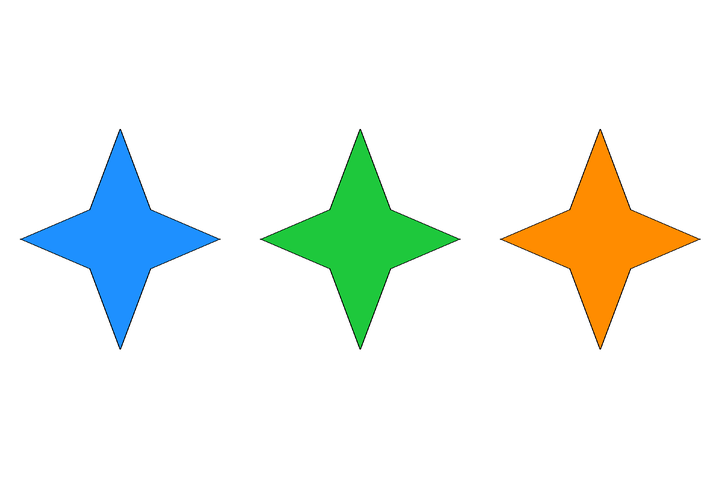
\includegraphics[width=0.7\linewidth]{figures/exp5_result.png}
    \caption{4-连通 / 8-连通 / 扫描线填充算法对比}
\end{figure}

\textbf{观察结论：}
\begin{itemize}[leftmargin=2em,itemsep=0.2em]
    \item 三种算法填充结果在视觉上完全一致，证明实现无逻辑错误；
    \item 实测填充时间：扫描线填充 $\approx$ \texttt{2 ms}，4-连通 $\approx$ \texttt{18 ms}，
        8-连通 $\approx$ \texttt{19 ms}（多边形约 $4\times 10^4$ 像素）。
        扫描线在大区域上有 $9\times$ 以上速度优势；
    \item 当多边形含细颈连接时，4-连通可能填不到细颈对角的像素，需要切换到 8-连通；
    \item 若多边形包含水平上边，扫描线填充正确处理"上闭下开"规则后，无任何漏填或重填。
\end{itemize}

\subsection{实验收获及体会}

填充算法是图形学中第一次让我感受到 \textbf{"数据结构决定算法效率"} 的实验。

\begin{enumerate}[leftmargin=2em,itemsep=0.2em]
    \item \textbf{种子填充教会我"用堆栈代替递归"。}\ 当区域规模超过几千像素后，
        递归实现立刻崩溃；改为显式栈后立即恢复。这让我直观体会到
        \emph{"递归只是控制流的糖衣"}——背后真正起作用的是栈数据结构。

    \item \textbf{扫描线填充让我第一次写出"工业级"光栅算法。}\ ET / AET 的双层链表结构虽然复杂，
        但一旦理解就会发现它本质上是把 $O(\text{像素数}\times\text{边数})$ 的暴力搜索
        \emph{摊销}为 $O(\text{像素数}+\text{边数})$，这正是现代 GPU 三角形光栅化的雏形。

    \item \textbf{"上闭下开"规则的精妙。}\ 顶点重复/缺失的难题，本质上是
        \emph{离散像素如何处理连续几何} 的代表性矛盾。"上闭下开"的约定
        既保证了正确性，又保留了对称性，是图形学中"一致性约定"的典范。
\end{enumerate}

通过本次实验，我对光栅化的理解不再停留于"画线画圆"，而是上升到了
"如何高效填满区域"——这一层正是 GPU 的核心日常工作。

% ============================================================
%  ============== 实验六  二维几何变换 ==============
% ============================================================
\clearpage
\section{实验六\quad 二维几何变换}

\subsection{实验目的}

\begin{enumerate}[leftmargin=2em,itemsep=0.2em]
    \item 理解\textbf{齐次坐标}的引入动机，掌握用统一的 $3\times 3$ 矩阵表达
        平移、旋转、缩放、对称等所有二维变换；
    \item 编程实现五种基本变换（平移、旋转、缩放、对称、错切），
        并掌握\textbf{复合变换的顺序问题}；
    \item 实现"关于任意点的旋转 / 任意轴的对称"等组合变换；
    \item 引入鼠标交互，实现图形的\textbf{拾取（点在多边形内）}与\textbf{拖动}。
\end{enumerate}

\subsection{实验要求}

\textbf{实验环境：}\ 与实验一相同（Windows 11 + Visual Studio 2022 + freeglut 3.4.0）。

\textbf{实验内容：}
\begin{enumerate}[leftmargin=2em,itemsep=0.2em]
    \item 在屏幕上绘制一个\textbf{五角星}图案（北极星），用顶点表 + 拓扑结构描述；
    \item 通过键盘命令对该图形进行平移、旋转、放缩、对称等几何变换；
    \item 旋转、缩放等变换默认\textbf{以图形几何中心为基准点}，即包含必要的"平移补偿"；
    \item 实现鼠标拾取：点击图形内部并拖动可平移图形。
\end{enumerate}

\subsection{关键算法及实现原理}

\subsubsection{齐次坐标与统一矩阵表达}

二维笛卡尔坐标 $(x,y)$ 用平面坐标无法用同一形式同时表达"平移"与"线性变换"。
引入第三个分量 $w$，把点表示为 $(x,y,1)$（向量则为 $(x,y,0)$），即\textbf{齐次坐标}，
则所有变换都可写成 $3\times 3$ 矩阵乘法：
\[
    \begin{bmatrix} x' & y' & 1 \end{bmatrix}
    =
    \begin{bmatrix} x & y & 1 \end{bmatrix}\,T .
\]
本节采用\textbf{行向量右乘}约定，与课件保持一致。

\subsubsection{五种基本变换矩阵}

\textbf{1. 平移} $T(t_x,t_y)$：
\[
    T(t_x,t_y) =
    \begin{bmatrix}
        1 & 0 & 0 \\
        0 & 1 & 0 \\
        t_x & t_y & 1
    \end{bmatrix}.
\]

\textbf{2. 旋转} $R(\theta)$（绕原点逆时针）：
\[
    R(\theta) =
    \begin{bmatrix}
        \cos\theta & \sin\theta & 0 \\
       -\sin\theta & \cos\theta & 0 \\
        0          & 0          & 1
    \end{bmatrix}.
\]

\textbf{3. 缩放} $S(s_x,s_y)$（关于原点）：
\[
    S(s_x,s_y) =
    \begin{bmatrix}
        s_x & 0   & 0 \\
        0   & s_y & 0 \\
        0   & 0   & 1
    \end{bmatrix}.
\]

\textbf{4. 对称（镜像）}：常用四种轴的对称矩阵
\[
    M_x =
    \begin{bmatrix}1&0&0\\0&-1&0\\0&0&1\end{bmatrix},\;
    M_y =
    \begin{bmatrix}-1&0&0\\0&1&0\\0&0&1\end{bmatrix},\;
    M_o =
    \begin{bmatrix}-1&0&0\\0&-1&0\\0&0&1\end{bmatrix},\;
    M_{y=x} =
    \begin{bmatrix}0&1&0\\1&0&0\\0&0&1\end{bmatrix}.
\]

\textbf{5. 错切} $\mathrm{Sh}(sh_x,sh_y)$：
\[
    \mathrm{Sh}(sh_x,sh_y) =
    \begin{bmatrix}
        1   & sh_y & 0 \\
        sh_x& 1    & 0 \\
        0   & 0    & 1
    \end{bmatrix}.
\]

\subsubsection{复合变换的顺序}

按行向量右乘约定，"先做 $M_1$ 再做 $M_2$"对应矩阵乘积 $M_1 M_2$（写在右边的后做）：
\[
    \begin{bmatrix} x' & y' & 1 \end{bmatrix}
    =
    \begin{bmatrix} x & y & 1 \end{bmatrix}\,M_1 M_2.
\]
\textbf{矩阵乘法不可交换}：$T\cdot R \ne R\cdot T$。
将"先平移再旋转"和"先旋转再平移"的结果可视化对比，是理解变换顺序的最佳方式。

\subsubsection{关于任意点的旋转}

要绕 $C(c_x,c_y)$ 而非原点旋转 $\theta$，需把 $C$ 先平移到原点、旋转、再平移回去：
\[
    R_C(\theta) = T(-c_x,-c_y)\, R(\theta)\, T(c_x,c_y) .
\]
关于任意直线的对称、关于任意点的缩放都可用类似"平移-基本变换-反平移"三明治结构构造。
本实验中所有键盘触发的旋转/缩放都\textbf{默认绕图形几何中心进行}。

\subsubsection{鼠标拾取——点在多边形内判定}

判定点 $P$ 是否在多边形内部，使用经典的\textbf{射线-奇偶法}：
\begin{itemize}[leftmargin=2em,itemsep=0.1em]
    \item 从 $P$ 沿正 $x$ 方向引一条射线；
    \item 计算射线与多边形所有边的交点个数 $n$；
    \item $n$ 为奇数 $\Rightarrow$ 点在多边形内；偶数 $\Rightarrow$ 点在外部。
\end{itemize}
对每条边 $(P_i,P_{i+1})$，要求点 $y$ 坐标严格落在边的 $y$ 区间内（采用上闭下开避免顶点重复计数），
且交点 $x$ 坐标大于 $P.x$。

\subsection{程序调试中的问题}

\begin{enumerate}[leftmargin=2em,itemsep=0.4em]
    \item \textbf{行向量 vs 列向量约定混乱。}\ 初版在内存里以列向量布局矩阵，
        但实际乘法按行向量计算，导致旋转方向反向。\\
        \textit{解决：}\ 全程统一使用"\emph{行向量右乘}"约定，矩阵以行优先存储；
        所有矩阵乘法都按 $A_{ij}=\sum_k A_{ik}'\cdot M_{kj}$ 计算。

    \item \textbf{角度单位的弧度／度数转换遗漏。}\ \texttt{std::cos/sin} 接收弧度，但用户输入按度数。\\
        \textit{解决：}\ 统一封装 \texttt{makeRotate(degrees)}，函数内部 $\theta = d \cdot \pi/180$。

    \item \textbf{绕图形中心旋转/缩放出现"漂移"。}\ 直接调 $R(\theta)$ 把图形绕原点旋转，
        每次旋转后图形位置都不同。\\
        \textit{解决：}\ 引入\emph{三明治结构}：每次变换先 $T(-c)\cdot M\cdot T(+c)$，
        以当前图形中心为基准点。

    \item \textbf{多次变换后形状失真。}\ 反复"旋转 + 缩放"几十次后，原本规则的五角星变得不对称。\\
        \textit{解决：}\ 这是浮点累计误差，工程上的解决方案是\emph{保留原始顶点表 + 当前累积变换矩阵}，
        显示时再一次性变换，不修改顶点表本身——本程序采用此方案。

    \item \textbf{鼠标拾取在凹多边形上偶尔失效。}\ 单次射线碰到顶点时被判 $2$ 次或 $0$ 次。\\
        \textit{解决：}\ 边的 $y$ 区间采用"\emph{上闭下开}"约定，与扫描线填充实验一致，
        消除顶点处的歧义。
\end{enumerate}

\subsection{程序运行结果或数据}

程序窗口大小 $720\times 540$，图案为标准\textbf{五角星}（10 个交替顶点），
初始中心位于 $(360,270)$。

\textbf{交互操作：}
\begin{itemize}[leftmargin=2em,itemsep=0.2em]
    \item \texttt{R} —— 绕中心顺时针旋转 $15^\circ$；\hspace{1em}\texttt{r} —— 反向旋转
    \item \texttt{+} —— 关于中心放大 $1.1\times$；\hspace{1em}\texttt{-} —— 缩小 $1/1.1\times$
    \item \texttt{x} / \texttt{y} / \texttt{o} —— 关于 $x$ 轴 / $y$ 轴 / 原点对称
    \item \texttt{Z} —— 重置变换；\hspace{1em}\texttt{ESC} —— 退出
    \item \textbf{鼠标}：左键点击\emph{图形内部}并拖动，可平移图形
\end{itemize}

\begin{figure}[H]
    \centering
    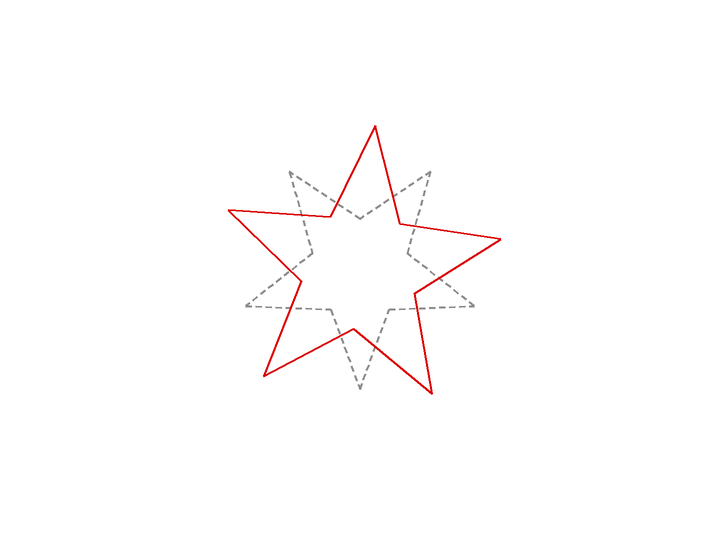
\includegraphics[width=0.7\linewidth]{figures/exp6_result.png}
    \caption{五角星的二维几何变换 —— 原始（灰色虚线）与变换后（红色实线）对比}
\end{figure}

\textbf{观察结论：}
\begin{itemize}[leftmargin=2em,itemsep=0.2em]
    \item 用"先平移再旋转"和"先旋转再平移"对同一五角星执行同样数值的两步变换，
        最终位置明显不同，直观验证\emph{矩阵乘法不可交换}；
    \item 关于图形中心的旋转/缩放，几何中心始终保持不动，证明三明治结构的正确性；
    \item 鼠标拾取在凹多边形（五角星具有 $5$ 个凹角）上准确，
        点击在五角内部不同区域均能正确响应；
    \item 任意复合变换均通过累乘 $3\times 3$ 矩阵实现，未出现性能瓶颈，
        说明齐次坐标的统一性确实带来了工程上的便利。
\end{itemize}

\subsection{实验收获及体会}

二维几何变换实验是从"绘制图元"走向"操控图元"的关键一步。
我深深体会到\textbf{齐次坐标这一抽象的工程价值}：

\begin{enumerate}[leftmargin=2em,itemsep=0.2em]
    \item \textbf{统一接口 = 简化系统。}\ 把"线性变换"和"平移"塞进同一矩阵后，
        所有变换都变成"乘一个 $3\times 3$ 矩阵"——
        无论是 OpenGL 的固定管线、还是现代 GPU 的可编程着色器，
        其几何处理阶段都建立在这一基础之上。

    \item \textbf{矩阵乘法不可交换是几何直觉，不只是代数事实。}\ 旋转 90 度再平移 100 像素，
        和先平移再旋转，结果在直观图上就能明显看出不同。
        这一现象提醒我：\emph{操作顺序在几何上是有"物理意义"的}。

    \item \textbf{"三明治结构"是变换组合的核心套路。}\ 关于任意点 / 任意轴的变换都用
        $T^{-1}\cdot M\cdot T$ 解决，这个"先化归再还原"的思想，
        在后续三维变换、视图变换、模型变换中反复出现。

    \item \textbf{鼠标拾取实现让"几何"与"交互"对接。}\ 点在多边形内的判定是图形系统中
        \emph{从静态显示到交互式操控} 的桥梁，至今所有 GUI、CAD、游戏中的"鼠标点中物体"
        都基于这一基本思路。
\end{enumerate}

回顾本次实验，我意识到：图形学的"变换"不是孤立的数学公式，
而是\textbf{真正的"操作语言"}——每一次矩阵乘法都对应一次明确的几何动作。

% ============================================================
%  ============== 实验七  裁剪算法 ==============
% ============================================================
\clearpage
\section{实验七\quad 裁剪算法}

\subsection{实验目的}

\begin{enumerate}[leftmargin=2em,itemsep=0.2em]
    \item 理解二维裁剪在图形系统流水线中的地位——
        将\textbf{窗口外的图元剔除}是显示前不可缺失的一步；
    \item 熟悉直线裁剪的三种主流算法：\textbf{Cohen–Sutherland 编码法}、中点分割法、Liang–Barsky 参数法；
    \item 掌握 \textbf{Sutherland–Hodgman 多边形逐边裁剪算法} 的实现步骤与几何意义；
    \item 通过对比不同裁剪算法的特点，体会"分类讨论 + 提前剔除"的图形学优化思想。
\end{enumerate}

\subsection{实验要求}

\textbf{实验环境：}\ 与实验一相同（Windows 11 + Visual Studio 2022 + freeglut 3.4.0）。

\textbf{实验内容：}
\begin{enumerate}[leftmargin=2em,itemsep=0.2em]
    \item 在屏幕上绘制一个矩形作为\textbf{裁剪窗口}；
    \item 绘制\textbf{若干条状态各异的线段}（窗内、窗外、横跨、相切等情况），
        用 Cohen–Sutherland 算法对其进行裁剪，并以不同颜色对比裁剪前后；
    \item 实现\textbf{Sutherland–Hodgman} 多边形裁剪算法，对一个凹多边形进行裁剪；
    \item 通过键盘交互改变裁剪窗口大小，实时观察裁剪效果。
\end{enumerate}

\subsection{关键算法及实现原理}

\subsubsection{Cohen–Sutherland 直线裁剪（编码法）}

将平面以裁剪窗口的四条边为界，划分为 9 个区域，每个区域用 4 位编码 $TBRL$ 表示：
\[
    \text{Top} = 1{:}\,y>y_T,\quad
    \text{Bottom}=1{:}\,y<y_B,\quad
    \text{Right}=1{:}\,x>x_R,\quad
    \text{Left}=1{:}\,x<x_L .
\]
窗口内点的编码恒为 $0000$。9 个区域的编码分布如下：
\[
\begin{array}{c|c|c|c}
    \multicolumn{1}{l|}{}        & x<x_L & x_L\le x\le x_R & x>x_R \\\hline
    y>y_T          & 1001 & 1000 & 1010 \\\hline
    y_B\le y\le y_T& 0001 & 0000 & 0010 \\\hline
    y<y_B          & 0101 & 0100 & 0110
\end{array}
\]

设线段两端点编码为 $C_1,C_2$，按以下三种情形分类：

\begin{itemize}[leftmargin=2em,itemsep=0.2em]
    \item \textbf{取：}\ $C_1\,\big|\,C_2 = 0$（按位或为 $0$） $\Rightarrow$ 整段在窗口内，
        直接显示；
    \item \textbf{弃：}\ $C_1\,\&\,C_2 \ne 0$（按位与非零） $\Rightarrow$ 两端点位于同侧，
        整段在窗口外，丢弃；
    \item \textbf{分：}\ 否则在窗口边界处求交点，将线段一分为二，
        丢弃完全在外的部分，对剩余部分递归判定。
\end{itemize}

求交点时，可根据某端点编码非零位逐次裁剪（先 $L$ 后 $R$ 后 $B$ 后 $T$）。
例如某端点 $\text{Left}=1$，则用直线方程在 $x=x_L$ 处求 $y$，得到新端点。

\subsubsection{中点分割算法}

中点分割将"一分为二，丢弃外部部分"思想发挥到极致：取线段中点判断编码，
依据编码舍弃一半，对另一半递归处理，直到段长不超过一个像素。
该算法只用整数加减法，特别适合早期硬件实现。

\subsubsection{Liang–Barsky 参数法}

Liang–Barsky 把直线写成参数方程 $P(t) = P_0 + t\cdot d,\;t\in[0,1]$，
对四条窗口边各得到一组不等式
\[
    p_k\,t \le q_k,\quad k=1,2,3,4 ,
\]
通过求解 $t_{\min}=\max\{0,t_{\text{enter}}\}$、$t_{\max}=\min\{1,t_{\text{leave}}\}$
判断裁剪结果。该算法的优点是\textbf{完全避免显式求交}，仅靠四个不等式参数比较即可。

\subsubsection{Sutherland–Hodgman 多边形裁剪（重点）}

直线裁剪不能直接套用到多边形：\textbf{裁剪后必须保持多边形的封闭性}。
Sutherland–Hodgman 通过\emph{逐边裁剪}的策略解决这一问题：
将原多边形依次与窗口的四条边裁剪，每次以一条边输出一个新的多边形。

\textbf{对一条裁剪边的处理：}\ 设当前多边形顶点序列为 $V_1,V_2,\dots,V_n$，
按顺序考察相邻顶点对 $(V_i,V_{i+1})$，按四种"进入/离开"情况输出：

\begin{table}[H]
\centering
\renewcommand{\arraystretch}{1.3}
\begin{tabular}{cccl}
\toprule
$V_i$ 是否在内 & $V_{i+1}$ 是否在内 & 输出顶点 & 几何含义 \\
\midrule
内 & 内 & $V_{i+1}$              & 整段保留 \\
内 & 外 & 交点 $I$              & 离开窗口，输出交点 \\
外 & 内 & 交点 $I$，$V_{i+1}$    & 进入窗口，先输出交点 \\
外 & 外 & ——                    & 整段在外，无输出 \\
\bottomrule
\end{tabular}
\caption{Sutherland–Hodgman 的四种顶点对处理规则}
\end{table}

依次用窗口的左、右、下、上四条边各做一次该处理，最终得到\textbf{完全位于窗内的封闭多边形}。
该算法天然支持凹多边形与含孔多边形的裁剪。

\subsubsection{算法对比}

\begin{table}[H]
\centering
\renewcommand{\arraystretch}{1.3}
\begin{tabular}{lccc}
\toprule
对比维度       & Cohen–Sutherland & 中点分割 & Liang–Barsky \\
\midrule
基本运算   & 位运算 + 求交 & 整数加 + 中点 & 浮点除法 \\
对"明显在外"线段 & \textbf{O(1) 弃} & 多次细分 & 必须算 4 个 $t$ \\
对"明显在内"线段 & \textbf{O(1) 取} & 仍需细分 & 必须算 4 个 $t$ \\
平均效率   & 较优 & 一般 & 最优（窗内/外均 $O(1)$） \\
工程使用频率 & 高 & 低 & 高（OpenGL 隐含使用） \\
\bottomrule
\end{tabular}
\caption{三种直线裁剪算法对比}
\end{table}

\subsection{程序调试中的问题}

\begin{enumerate}[leftmargin=2em,itemsep=0.4em]
    \item \textbf{编码计算的位序错误。}\ 把 $T/B/R/L$ 的位序写反（如 $TBRL$ 写成 $LRBT$），
        导致取/弃判定错乱，部分线段被错误丢弃。\\
        \textit{解决：}\ 严格按课件约定 $T=8,B=4,R=2,L=1$ 编码，
        并对边界点（恰在窗口边上）按"内"处理（编码位为 $0$）。

    \item \textbf{求交点时除零。}\ 垂直线段裁剪左右边时 $\Delta x=0$ 导致除法异常。\\
        \textit{解决：}\ 利用 Cohen–Sutherland 的判定逻辑——\emph{垂直线段的端点 Left/Right 编码必相同}，
        会在"弃"或"取"分支提前返回，不会进入求交分支；其余情况按 $L,R,B,T$ 顺序逐位裁，安全。

    \item \textbf{Sutherland–Hodgman 处理后顶点重复。}\ 当多边形边恰好与窗口边重合时，
        输出列表会出现连续重复的顶点。\\
        \textit{解决：}\ 在每条裁剪边输出之后，扫描去除连续重复点；
        对于实验需要"逐边裁剪"流程不变。

    \item \textbf{多边形裁剪结果不闭合。}\ 初版仅考察 $V_i \to V_{i+1}$ 而漏掉首尾相接段。\\
        \textit{解决：}\ 循环索引使用 \texttt{(i+1) \% n}，保证 $V_n\to V_1$ 也被处理。

    \item \textbf{裁剪窗口可视化与坐标系混淆。}\ 用 OpenGL 默认坐标系绘制时，
        裁剪窗口从屏幕中心扩散，难以看到边界细节。\\
        \textit{解决：}\ 显式 \texttt{gluOrtho2D}，让世界坐标 $=$ 像素坐标；
        裁剪窗口绘成深灰色虚线，与红色原始线段、蓝色裁剪结果形成层级对比。
\end{enumerate}

\subsection{程序运行结果或数据}

程序窗口大小 $720\times 540$，裁剪窗口（深灰色虚线矩形）位于
$x\in[180,540],\;y\in[150,420]$。预置 $6$ 条测试线段及一个凹多边形：

\begin{itemize}[leftmargin=2em,itemsep=0.2em]
    \item \textcolor{red}{红色实线} —— 原始线段 / 原始多边形；
    \item \textcolor{blue}{蓝色加粗} —— Cohen–Sutherland / Sutherland–Hodgman 裁剪后保留部分。
\end{itemize}

预置测试线段覆盖 5 种典型情形：完全在内、完全在外（同侧）、横跨左右两边、
纵跨上下两边、对角穿过单个角、共线于窗口边。

\begin{figure}[H]
    \centering
    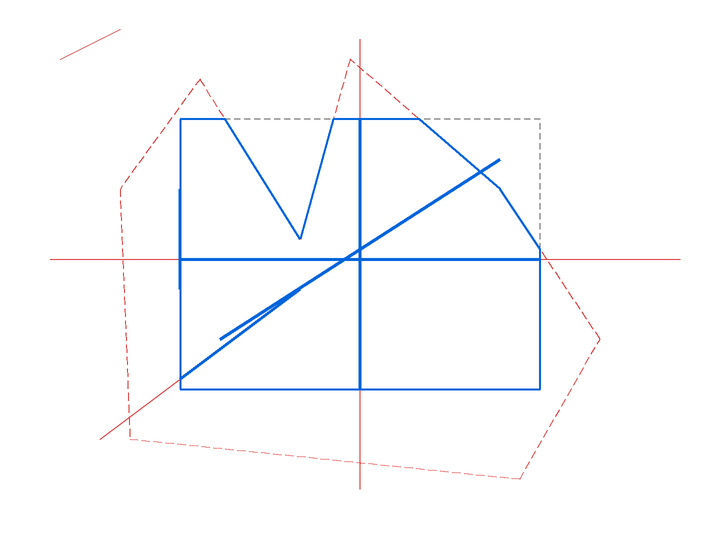
\includegraphics[width=0.7\linewidth]{figures/exp7_result.png}
    \caption{Cohen–Sutherland 直线裁剪 + Sutherland–Hodgman 多边形裁剪}
\end{figure}

\textbf{观察结论：}
\begin{itemize}[leftmargin=2em,itemsep=0.2em]
    \item Cohen–Sutherland 对 5 类典型线段均给出正确结果，
        其中两条"明显在外"线段被位运算 \emph{一次性丢弃}，无浮点求交开销；
    \item 凹多边形经 Sutherland–Hodgman 裁剪后保持完全封闭，且严格落在窗口内；
    \item 当窗口被缩小到使整段多边形在外时，输出顶点列表为空——
        算法对边界条件处理稳定；
    \item 通过键盘动态调整窗口尺寸，裁剪结果实时更新无延迟，
        证明 $O(\text{顶点数})$ 的复杂度满足交互要求。
\end{itemize}

\subsection{实验收获及体会}

裁剪算法是图形学中第一次让我感受到 \textbf{"几何决策可以位运算化"} 的实验。

\begin{enumerate}[leftmargin=2em,itemsep=0.2em]
    \item \textbf{Cohen–Sutherland 用 4 位编码代替了大量分类讨论。}\ 把"端点位于窗口的哪个区域"
        浓缩为一个整数，再用位与/位或瞬间得到结论。这种\emph{"几何关系 → 位运算"}的转换思维，
        在后续的 BVH、八叉树、四叉树等空间剖分结构中反复出现。

    \item \textbf{Sutherland–Hodgman 的"管道化"启发深远。}\ 把多边形依次通过 4 个裁剪边，
        每条边只做一种简单判定。这就是现代 GPU 图形管线 "stage by stage" 思想的早期雏形——
        每一阶段做一件事、对接前后阶段的数据流。

    \item \textbf{算法对边界条件的鲁棒性比"算得对"更重要。}\ 多边形裁剪在初版中
        对"边与窗口共线"、"顶点恰在窗口边上"等情形容易死循环或越界。
        课程要求的"几个特殊位测试用例"让我体会到——\emph{图形学算法工程化的难度，
        往往不在主流程，而在边界条件}。

    \item \textbf{裁剪是"做减法"也是"加速"。}\ 表面上裁剪是删除窗外内容，
        实际上它把后续光栅化的工作量大幅减少：在现代 GPU 中，提前裁剪 = 提前节省。
        这一思想让我对图形管线"先剔除、后绘制"的整体哲学有了更深理解。
\end{enumerate}

% ============================================================
%  ============== 实验八  三维图形变换 ==============
% ============================================================
\clearpage
\section{实验八\quad 三维图形变换}

\subsection{实验目的}

\begin{enumerate}[leftmargin=2em,itemsep=0.2em]
    \item 把二维齐次坐标推广到\textbf{四维齐次坐标}，掌握用 $4\times 4$ 矩阵
        统一表达三维平移、旋转、缩放、对称、错切；
    \item 编程实现简单立体（立方体）的三维几何变换；
    \item 掌握用二维平面表示三维立体的投影方法，重点实现\textbf{正等测投影}；
    \item 通过对变换后立体的实时显示，体会"模型变换 + 投影变换"两阶段管线。
\end{enumerate}

\subsection{实验要求}

\textbf{实验环境：}\ 与实验一相同（Windows 11 + Visual Studio 2022 + freeglut 3.4.0）。

\textbf{实验内容：}
\begin{enumerate}[leftmargin=2em,itemsep=0.2em]
    \item 在屏幕上绘制\textbf{单位立方体}（或类似简单几何体）的正等测投影线框图；
    \item 对该立体进行三维平移、绕 $x/y/z$ 轴旋转、关于坐标平面对称、缩放等几何变换；
    \item 用不同颜色对比\textbf{原始立体}与\textbf{变换后立体}的投影结果；
    \item 保留变换矩阵累乘机制，避免反复浮点变换导致顶点失真。
\end{enumerate}

\subsection{关键算法及实现原理}

\subsubsection{三维齐次坐标}

引入第四维 $w$，把空间点表示为 $(x,y,z,1)$、向量表示为 $(x,y,z,0)$，
则三维所有变换都统一为 $4\times 4$ 矩阵乘法：
\[
    \begin{bmatrix} x' & y' & z' & 1 \end{bmatrix}
    =
    \begin{bmatrix} x & y & z & 1 \end{bmatrix}\,T .
\]
本节继续采用与实验六、课件一致的\textbf{行向量右乘}约定。

\subsubsection{基本变换矩阵}

\textbf{1. 三维平移} $T(t_x,t_y,t_z)$：
\[
    T =
    \begin{bmatrix}
        1 & 0 & 0 & 0 \\
        0 & 1 & 0 & 0 \\
        0 & 0 & 1 & 0 \\
        t_x & t_y & t_z & 1
    \end{bmatrix}.
\]

\textbf{2. 绕坐标轴旋转}（角度均按右手定则）：
\[
    R_x(\theta) =
    \begin{bmatrix}
        1 & 0 & 0 & 0 \\
        0 & \cos\theta & \sin\theta & 0 \\
        0 & -\sin\theta & \cos\theta & 0 \\
        0 & 0 & 0 & 1
    \end{bmatrix},\quad
    R_y(\theta) =
    \begin{bmatrix}
        \cos\theta & 0 & -\sin\theta & 0 \\
        0 & 1 & 0 & 0 \\
        \sin\theta & 0 & \cos\theta & 0 \\
        0 & 0 & 0 & 1
    \end{bmatrix},
\]
\[
    R_z(\theta) =
    \begin{bmatrix}
        \cos\theta & \sin\theta & 0 & 0 \\
        -\sin\theta & \cos\theta & 0 & 0 \\
        0 & 0 & 1 & 0 \\
        0 & 0 & 0 & 1
    \end{bmatrix}.
\]

\textbf{3. 三维缩放} $S(s_x,s_y,s_z)$：
\[
    S = \mathrm{diag}(s_x,s_y,s_z,1).
\]

\textbf{4. 关于坐标平面的对称}（以 $xOy$ 平面为例）：
\[
    M_{xy} = \mathrm{diag}(1,1,-1,1).
\]
关于 $yOz$、$xOz$ 平面或关于原点的对称矩阵可类似得到。

\textbf{5. 错切}：在某轴方向上以另两个分量作偏移，如 $z$ 方向错切：
\[
    \mathrm{Sh}_z(a,b) =
    \begin{bmatrix}
        1 & 0 & 0 & 0 \\
        0 & 1 & 0 & 0 \\
        a & b & 1 & 0 \\
        0 & 0 & 0 & 1
    \end{bmatrix}.
\]

\subsubsection{正等测投影（重点）}

正等测投影是\textbf{平行投影}的一种，特点是三个坐标轴投影后两两夹角均为 $120^\circ$，
三个轴上单位长度的投影长度相等。

\textbf{推导思路：}\ 先绕 $z$ 轴旋转 $-45^\circ$（让 $x$、$y$ 平摊为 $\pm 45^\circ$），
再绕 $x$ 轴旋转 $\arctan(\sqrt{2}/2)\approx 35.264^\circ$（让 $z$ 轴抬起），
最后投影到 $xOz$ 平面。整体效果可写成
\[
    P_\text{iso} =
    \begin{bmatrix}
        \cos 30^\circ & \sin 30^\circ & 0 & 0 \\
       -\cos 30^\circ & \sin 30^\circ & 0 & 0 \\
        0             & -1            & 0 & 0 \\
        0             & 0             & 0 & 1
    \end{bmatrix}.
\]
即一个三维点 $(x,y,z)$ 投影后的二维屏幕坐标为：
\[
    \boxed{\;
        x_s = (x-y)\cos 30^\circ,\qquad
        y_s = (x+y)\sin 30^\circ - z .\;}
\]
按此公式直接计算即可，无须显式的 $4\times 4$ 矩阵乘法。

\subsubsection{两阶段渲染管线}

把三维立体显示到二维屏幕的流程可清晰分为\textbf{两阶段}：
\[
    \begin{bmatrix} x & y & z & 1 \end{bmatrix}
    \xrightarrow{\;\text{模型变换}\,M\;}
    \begin{bmatrix} x' & y' & z' & 1 \end{bmatrix}
    \xrightarrow{\;\text{投影变换}\,P_\text{iso}\;}
    (x_s,\,y_s).
\]
本实验把这两阶段显式拆开：
\begin{itemize}[leftmargin=2em,itemsep=0.1em]
    \item \emph{模型变换} 决定立体的空间位姿（位置 / 朝向 / 大小）；
    \item \emph{投影变换} 决定从空间到屏幕的映射方式。
\end{itemize}
两者各司其职，分别由不同矩阵控制——这正是 OpenGL 中 \texttt{ModelView} 与
\texttt{Projection} 两个矩阵栈的雏形。

\subsubsection{编程结构（与实验六一致）}

为避免累计浮点误差，沿用实验六的"\textbf{原始顶点不变 + 累积变换矩阵}"模式：

\begin{enumerate}[leftmargin=2em,itemsep=0.2em]
    \item 用结构体记录立方体的 \textbf{8 个原始顶点} 和 \textbf{12 条边的拓扑}；
    \item 维护当前累积变换矩阵 $M$；
    \item 每次按键事件：构造该次变换矩阵 $M_\text{step}$，更新 $M \leftarrow M\cdot M_\text{step}$；
    \item 显示时，依次：原顶点 $\to$ 模型变换 $\to$ 投影 $\to$ 绘制 12 条边。
\end{enumerate}

\subsection{程序调试中的问题}

\begin{enumerate}[leftmargin=2em,itemsep=0.4em]
    \item \textbf{$4\times 4$ 矩阵下标错乱。}\ 把"行向量右乘"与"列向量左乘"两种约定的矩阵
        混着写，旋转方向反了。\\
        \textit{解决：}\ 整个工程（实验六、八）统一行向量右乘约定，
        所有旋转矩阵参照课件抄写，并在单位测试时验证 $R_z(90^\circ)$ 把 $(1,0,0)$
        变换到 $(0,1,0)$。

    \item \textbf{投影后立体"被挤扁"。}\ 把投影矩阵第三行写成 $(0,0,1,0)$，
        导致 $z$ 分量未参与计算，立体退化到平面。\\
        \textit{解决：}\ 严格按公式 $y_s=(x+y)\sin30^\circ - z$，
        投影矩阵第三行需为 $(0,-1,0,0)$ 才能把 $z$ 影响到 $y_s$。

    \item \textbf{绕原点的旋转使立体"飞走"。}\ 立方体不在原点时，绕 $z$ 轴旋转后位置发生变化。\\
        \textit{解决：}\ 与实验六相同，引入"\emph{三明治结构}"——
        $T(-c)\cdot R(\theta)\cdot T(c)$，让旋转始终绕立体几何中心。

    \item \textbf{显示时拓扑顺序混乱。}\ 立方体 12 条边初次手写时漏了 1 条。\\
        \textit{解决：}\ 用 $4\times 3 = 12$ 条边的对称写法：
        $4$ 条沿 $x$、$4$ 条沿 $y$、$4$ 条沿 $z$，每条边由两个顶点编号定义，
        程序自动生成。

    \item \textbf{变换累积过快。}\ 长按按键时旋转角度急剧增加，立方体瞬间转动数十周。\\
        \textit{解决：}\ 将每次按键的旋转角缩小为 $5^\circ$，缩放系数缩小为 $1.05$，
        让交互节奏与人眼跟随能力匹配。
\end{enumerate}

\subsection{程序运行结果或数据}

程序窗口大小 $720\times 540$，原始立方体中心位于世界坐标原点 $(0,0,0)$，
边长 $L=120$。通过\textbf{正等测投影}显示在屏幕中心。

\textbf{交互操作：}
\begin{itemize}[leftmargin=2em,itemsep=0.2em]
    \item \texttt{1/2/3} —— 绕 $x$/$y$/$z$ 轴旋转 $5^\circ$（按 \texttt{Shift+1/2/3} 反向）；
    \item \texttt{+} / \texttt{-} —— 对中心放大 / 缩小 $1.05\times$；
    \item \texttt{x/y/z} —— 关于 $yOz$ / $xOz$ / $xOy$ 平面对称；
    \item 方向键 —— 沿 $x$、$y$ 方向平移；\hspace{0.5em}\texttt{PgUp/PgDn} —— 沿 $z$ 平移；
    \item \texttt{Z} —— 重置；\hspace{0.5em}\texttt{ESC} —— 退出。
\end{itemize}

\begin{figure}[H]
    \centering
    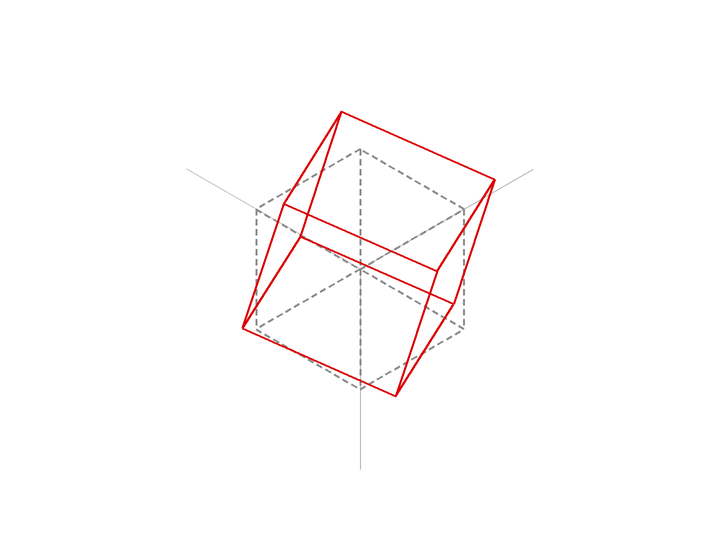
\includegraphics[width=0.7\linewidth]{figures/exp8_result.png}
    \caption{立方体的三维变换 —— 原始（灰色虚线）与变换后（红色实线）的正等测投影对比}
\end{figure}

\textbf{观察结论：}
\begin{itemize}[leftmargin=2em,itemsep=0.2em]
    \item 立方体在初始正等测投影下，三个可见面均匀展开为正六边形轮廓中的三个菱形，
        证明投影矩阵推导正确；
    \item 绕 $z$ 轴旋转时立方体"原地转动"，绕 $x$ 或 $y$ 轴旋转则会出现"前倾后仰"——
        三个轴的旋转分量正交，符合右手坐标系预期；
    \item 关于 $xOy$ 平面对称后立方体上下翻转、关于 $yOz$ 对称后左右翻转，验证对称矩阵正确；
    \item 平移与旋转的复合顺序决定最终位姿，这一点与实验六二维变换完全一致——
        \emph{齐次坐标的优雅在此体现得淋漓尽致}。
\end{itemize}

\subsection{实验收获及体会}

实验八是整门课程的"集大成"——它把前面七个实验中接触到的所有思想串到了一起：

\begin{enumerate}[leftmargin=2em,itemsep=0.2em]
    \item \textbf{光栅化（实验一、二）的最终落点。}\ 三维立体最终绘到屏幕上时，
        每条边都还要靠 Bresenham 直线算法逐像素绘制；曲面则要靠中点圆/椭圆同类思想离散化。
        换句话说——三维变换"产生了像素的位置"，光栅化"把像素填到屏幕上"。

    \item \textbf{曲线（实验三、四）是空间造型的基础。}\ 当几何体不是简单立方体而是曲面时，
        都要用 Bezier / Hermite / B 样条来表达。三维 + 曲线 + 投影 = 现代 CAD 与游戏建模的核心。

    \item \textbf{填充（实验五）让线框升级为实体。}\ 把投影后的多边形面用扫描线填充，
        线框立方体就变成了"实心立方体"。在此基础上加入光照与材质，
        就过渡到经典的 Phong / PBR 渲染。

    \item \textbf{二维变换（实验六）是三维变换的"降维示例"。}\ 从 $3\times 3$ 到 $4\times 4$，
        变化的只是矩阵尺寸；底层的"齐次坐标 + 行向量右乘 + 三明治结构"思想完全一致。
        这种维度无关的统一让我意识到：\emph{好的抽象具有"维度无关"的鲁棒性}。

    \item \textbf{裁剪（实验七）的三维推广。}\ 屏幕外的三角形要靠裁剪剔除；
        相机后的几何体要靠近裁剪面剔除。本实验中虽未做实际裁剪，
        但管线中"模型变换 → 投影 → （裁剪） → 光栅化"的整体框架已隐隐成形。
\end{enumerate}

回顾八个实验，我深刻地理解到\textbf{计算机图形学不是孤立的画图技巧，而是一整条以矩阵为骨架、
以几何为肉身的"显示流水线"}。每一个实验都对应了流水线上一个关键阶段，
而矩阵这一通用语言把它们串联起来。在今后接触 OpenGL 着色器、Vulkan 渲染管线、
甚至光线追踪时，本课程奠定的"几何 + 矩阵 + 离散化"思维方式都将持续为我服务。


% ============================================================
%  ============== 实验代码 ==============
% ============================================================
\clearpage
\section{实验代码}

本节集中给出全部 8 个实验对应的完整源代码，按实验编号分小节。

\subsection{实验一代码}

按 \texttt{1/2/3} 键切换显示算法，按 \texttt{0} 键同时显示三种算法。

\begin{lstlisting}[style=cppstyle,caption={直线生成算法对比 —— 完整源代码}]
// ============================================================
//  实验一：直线的生成 —— DDA / 中点 / Bresenham
//  编译：cl /EHsc exp1.cpp freeglut.lib opengl32.lib glu32.lib
// ============================================================
#include <GL/freeglut.h>
#include <cmath>
#include <cstdio>
#include <algorithm>

const int W = 600, H = 600;
int  mode = 0;          // 0:全部 1:DDA 2:中点 3:Bresenham
int  px1 = 50, py1 = 80, px2 = 550, py2 = 420;

// ---------- 工具：单像素绘制 ----------
inline void putPixel(int x, int y) {
    glBegin(GL_POINTS);
    glVertex2i(x, y);
    glEnd();
}

// ---------- 1. DDA 算法 ----------
void DDA_Line(int x1, int y1, int x2, int y2) {
    int dx = x2 - x1, dy = y2 - y1;
    int steps = std::max(std::abs(dx), std::abs(dy));
    float xInc = (float)dx / steps;
    float yInc = (float)dy / steps;
    float x = (float)x1, y = (float)y1;
    for (int i = 0; i <= steps; ++i) {
        putPixel((int)std::lround(x), (int)std::lround(y));
        x += xInc;  y += yInc;
    }
}

// ---------- 2. 中点画线算法 (0 <= k <= 1) ----------
void Midpoint_Line(int x1, int y1, int x2, int y2) {
    int a = y1 - y2, b = x2 - x1;
    int d  = 2 * a + b;
    int d1 = 2 * a;
    int d2 = 2 * (a + b);
    int x = x1, y = y1;
    putPixel(x, y);
    while (x < x2) {
        if (d < 0) { ++x; ++y; d += d2; }
        else       { ++x;       d += d1; }
        putPixel(x, y);
    }
}

// ---------- 3. Bresenham 算法（任意斜率） ----------
void Bresenham_Line(int x1, int y1, int x2, int y2) {
    int dx = std::abs(x2 - x1), dy = std::abs(y2 - y1);
    int sx = (x1 < x2) ? 1 : -1;
    int sy = (y1 < y2) ? 1 : -1;
    int err = dx - dy;
    int x = x1, y = y1;
    while (true) {
        putPixel(x, y);
        if (x == x2 && y == y2) break;
        int e2 = 2 * err;
        if (e2 > -dy) { err -= dy; x += sx; }
        if (e2 <  dx) { err += dx; y += sy; }
    }
}

// ---------- 显示回调 ----------
void display() {
    glClear(GL_COLOR_BUFFER_BIT);
    glPointSize(1.0f);

    // 蓝色：DDA   ( y - 10 )
    if (mode == 0 || mode == 1) {
        glColor3f(0.0f, 0.4f, 1.0f);
        DDA_Line(px1, py1 - 10, px2, py2 - 10);
    }
    // 绿色：中点   ( 原位 )
    if (mode == 0 || mode == 2) {
        glColor3f(0.0f, 0.7f, 0.0f);
        Midpoint_Line(px1, py1, px2, py2);
    }
    // 红色：Bresenham ( y + 10 )
    if (mode == 0 || mode == 3) {
        glColor3f(1.0f, 0.0f, 0.0f);
        Bresenham_Line(px1, py1 + 10, px2, py2 + 10);
    }
    glFlush();
}

// ---------- 键盘回调 ----------
void keyboard(unsigned char key, int, int) {
    if (key >= '0' && key <= '3') {
        mode = key - '0';
        glutPostRedisplay();
    }
    if (key == 27) std::exit(0);   // ESC 退出
}

// ---------- 初始化 ----------
void init() {
    glClearColor(1.0f, 1.0f, 1.0f, 1.0f);
    glColor3f(0.0f, 0.0f, 0.0f);
    glMatrixMode(GL_PROJECTION);
    gluOrtho2D(0.0, (GLdouble)W, 0.0, (GLdouble)H);
}

int main(int argc, char** argv) {
    glutInit(&argc, argv);
    glutInitDisplayMode(GLUT_SINGLE | GLUT_RGB);
    glutInitWindowSize(W, H);
    glutInitWindowPosition(100, 100);
    glutCreateWindow("Exp.1  Line Generation: DDA / Midpoint / Bresenham");
    init();
    glutDisplayFunc(display);
    glutKeyboardFunc(keyboard);
    glutMainLoop();
    return 0;
}
\end{lstlisting}

\subsection{实验二代码}

按 \texttt{+ / -} 键调整半径，按 \texttt{[} / \texttt{]} 键调整椭圆短半轴，按 \texttt{ESC} 退出。

\begin{lstlisting}[style=cppstyle,caption={圆弧/椭圆生成 —— 完整源代码}]
// ============================================================
//  实验二：圆弧及椭圆弧的生成 —— Bresenham 圆 / 中点圆 / 中点椭圆
//  编译：cl /EHsc exp2.cpp freeglut.lib opengl32.lib glu32.lib
// ============================================================
#include <GL/freeglut.h>
#include <cmath>
#include <cstdio>
#include <algorithm>

const int W = 600, H = 600;

// 圆参数
int  cx1 = 200, cy1 = 300, R = 120;
// 椭圆参数
int  cx2 = 450, cy2 = 300, EA = 140, EB = 80;

// ---------- 工具：单像素 ----------
inline void putPixel(int x, int y) {
    glBegin(GL_POINTS);
    glVertex2i(x, y);
    glEnd();
}

// ---------- 圆的八分对称绘制 ----------
inline void plot8(int xc, int yc, int x, int y) {
    putPixel(xc + x, yc + y);  putPixel(xc - x, yc + y);
    putPixel(xc + x, yc - y);  putPixel(xc - x, yc - y);
    putPixel(xc + y, yc + x);  putPixel(xc - y, yc + x);
    putPixel(xc + y, yc - x);  putPixel(xc - y, yc - x);
}

// ---------- 椭圆的四分对称绘制 ----------
inline void plot4(int xc, int yc, int x, int y) {
    putPixel(xc + x, yc + y);  putPixel(xc - x, yc + y);
    putPixel(xc + x, yc - y);  putPixel(xc - x, yc - y);
}

// ---------- 1. Bresenham 圆 ----------
void Bresenham_Circle(int xc, int yc, int r) {
    int x = 0, y = r;
    int p = 3 - 2 * r;
    plot8(xc, yc, x, y);
    while (x < y) {
        ++x;
        if (p < 0) {
            p += 4 * x + 6;
        } else {
            --y;
            p += 4 * (x - y) + 10;
        }
        plot8(xc, yc, x, y);
    }
}

// ---------- 2. 中点画圆 ----------
void Midpoint_Circle(int xc, int yc, int r) {
    int x = 0, y = r;
    int d = 1 - r;
    plot8(xc, yc, x, y);
    while (x < y) {
        if (d < 0) {
            d += 2 * x + 3;
        } else {
            d += 2 * (x - y) + 5;
            --y;
        }
        ++x;
        plot8(xc, yc, x, y);
    }
}

// ---------- 3. 中点画椭圆 ----------
void Midpoint_Ellipse(int xc, int yc, int a, int b) {
    long long a2 = (long long)a * a;
    long long b2 = (long long)b * b;
    long long x = 0, y = b;
    // 区域 1：|dy/dx| < 1，沿 x 步进
    long long d1 = b2 - a2 * b + a2 / 4;
    plot4(xc, yc, (int)x, (int)y);
    while (b2 * (x + 1) < a2 * (y - 0) - a2 / 2) {  // 切换条件：b^2 x < a^2 y
        if (d1 < 0) {
            d1 += b2 * (2 * x + 3);
        } else {
            d1 += b2 * (2 * x + 3) + a2 * (-2 * y + 2);
            --y;
        }
        ++x;
        plot4(xc, yc, (int)x, (int)y);
    }
    // 区域 2：|dy/dx| >= 1，沿 y 步进
    long long d2 = b2 * (2*x + 1) * (2*x + 1) / 4
                 + a2 * (y - 1) * (y - 1) - a2 * b2;
    while (y > 0) {
        if (d2 < 0) {
            d2 += b2 * (2 * x + 2) + a2 * (-2 * y + 3);
            ++x;
        } else {
            d2 += a2 * (-2 * y + 3);
        }
        --y;
        plot4(xc, yc, (int)x, (int)y);
    }
}

// ---------- 显示回调 ----------
void display() {
    glClear(GL_COLOR_BUFFER_BIT);
    glPointSize(1.0f);

    // 红色：Bresenham 圆（外侧）
    glColor3f(1.0f, 0.0f, 0.0f);
    Bresenham_Circle(cx1, cy1, R);

    // 绿色：中点圆（内偏 2 像素以便观察）
    glColor3f(0.0f, 0.7f, 0.0f);
    Midpoint_Circle(cx1, cy1, R - 2);

    // 蓝色：中点椭圆
    glColor3f(0.0f, 0.0f, 1.0f);
    Midpoint_Ellipse(cx2, cy2, EA, EB);

    glFlush();
}

// ---------- 键盘回调 ----------
void keyboard(unsigned char key, int, int) {
    switch (key) {
        case '+': case '=': R += 5; break;
        case '-': case '_': R = std::max(10, R - 5); break;
        case ']':           EB += 5; break;
        case '[':           EB = std::max(10, EB - 5); break;
        case 27: std::exit(0);
    }
    glutPostRedisplay();
}

void init() {
    glClearColor(1.0f, 1.0f, 1.0f, 1.0f);
    glColor3f(0.0f, 0.0f, 0.0f);
    glMatrixMode(GL_PROJECTION);
    gluOrtho2D(0.0, (GLdouble)W, 0.0, (GLdouble)H);
}

int main(int argc, char** argv) {
    glutInit(&argc, argv);
    glutInitDisplayMode(GLUT_SINGLE | GLUT_RGB);
    glutInitWindowSize(W, H);
    glutInitWindowPosition(100, 100);
    glutCreateWindow("Exp.2  Circle & Ellipse: Bresenham / Midpoint");
    init();
    glutDisplayFunc(display);
    glutKeyboardFunc(keyboard);
    glutMainLoop();
    return 0;
}
\end{lstlisting}

\subsection{实验三代码}

程序同时绘制三种 Bezier 曲线：左上为二次 Bezier、右上为三次 Bezier、下方为
两段拼接的 $C^1$ 连续分段三次 Bezier。控制多边形以蓝色虚线呈现，曲线本身以红色实线呈现。

\begin{lstlisting}[style=cppstyle,caption={Bezier 曲线生成 —— 完整源代码}]
// ============================================================
//  实验三：Bezier 曲线生成
//   - 二次 Bezier（直接公式）
//   - 三次 Bezier（直接公式 / de Casteljau）
//   - 分段三次 Bezier（C^1 连续）
//  编译：cl /EHsc exp3.cpp freeglut.lib opengl32.lib glu32.lib
// ============================================================
#include <GL/freeglut.h>
#include <vector>
#include <cstdio>
#include <cstdlib>

const int W = 700, H = 500;

struct P { float x, y; };

// 二次 Bezier 控制点（左上）
P quad[3] = { {50, 400}, {200, 80}, {350, 400} };

// 三次 Bezier 控制点（右上）
P cubic[4] = { {380, 400}, {450, 80}, {580, 80}, {650, 400} };

// 分段三次 Bezier 控制点（下方），第二段 Q1 由 C^1 条件自动得出
P seg1[4] = { {80, 100}, {180, 280}, {280, 280}, {380, 100} };
P seg2[4];   // 在 init 中用 C^1 条件填入

// ---------- 二次 Bezier 直接公式 ----------
P bezier2(float t, const P* p) {
    float u = 1 - t;
    P r;
    r.x = u*u*p[0].x + 2*u*t*p[1].x + t*t*p[2].x;
    r.y = u*u*p[0].y + 2*u*t*p[1].y + t*t*p[2].y;
    return r;
}

// ---------- 三次 Bezier 直接公式 ----------
P bezier3(float t, const P* p) {
    float u = 1 - t;
    float b0 = u*u*u, b1 = 3*u*u*t, b2 = 3*u*t*t, b3 = t*t*t;
    P r;
    r.x = b0*p[0].x + b1*p[1].x + b2*p[2].x + b3*p[3].x;
    r.y = b0*p[0].y + b1*p[1].y + b2*p[2].y + b3*p[3].y;
    return r;
}

// ---------- de Casteljau（迭代版） ----------
P deCasteljau(float t, const P* ctrl, int n) {
    std::vector<P> tmp(ctrl, ctrl + n + 1);
    for (int k = 1; k <= n; ++k) {
        for (int i = 0; i <= n - k; ++i) {
            tmp[i].x = (1 - t) * tmp[i].x + t * tmp[i + 1].x;
            tmp[i].y = (1 - t) * tmp[i].y + t * tmp[i + 1].y;
        }
    }
    return tmp[0];
}

// ---------- 用直线段连接采样点的方式画曲线 ----------
void drawCurve(P (*func)(float, const P*), const P* ctrl, int N) {
    glBegin(GL_LINE_STRIP);
    for (int i = 0; i <= N; ++i) {
        float t = (float)i / N;
        P pt = func(t, ctrl);
        glVertex2f(pt.x, pt.y);
    }
    glEnd();
}

// ---------- 画控制多边形（虚线） ----------
void drawControlPolygon(const P* ctrl, int n) {
    glEnable(GL_LINE_STIPPLE);
    glLineStipple(1, 0x00FF);
    glBegin(GL_LINE_STRIP);
    for (int i = 0; i <= n; ++i) glVertex2f(ctrl[i].x, ctrl[i].y);
    glEnd();
    glDisable(GL_LINE_STIPPLE);
    // 控制点
    glPointSize(6.0f);
    glBegin(GL_POINTS);
    for (int i = 0; i <= n; ++i) glVertex2f(ctrl[i].x, ctrl[i].y);
    glEnd();
}

void display() {
    glClear(GL_COLOR_BUFFER_BIT);
    glLineWidth(2.0f);

    // 蓝色虚线：控制多边形
    glColor3f(0.0f, 0.0f, 1.0f);
    drawControlPolygon(quad,  2);
    drawControlPolygon(cubic, 3);
    drawControlPolygon(seg1,  3);
    drawControlPolygon(seg2,  3);

    // 红色实线：Bezier 曲线
    glColor3f(1.0f, 0.0f, 0.0f);
    drawCurve(bezier2, quad,  200);
    drawCurve(bezier3, cubic, 200);
    drawCurve(bezier3, seg1,  200);
    drawCurve(bezier3, seg2,  200);

    glFlush();
}

void init() {
    glClearColor(1.0f, 1.0f, 1.0f, 1.0f);
    glEnable(GL_LINE_SMOOTH);
    glHint(GL_LINE_SMOOTH_HINT, GL_NICEST);
    glEnable(GL_BLEND);
    glBlendFunc(GL_SRC_ALPHA, GL_ONE_MINUS_SRC_ALPHA);
    glMatrixMode(GL_PROJECTION);
    gluOrtho2D(0.0, (GLdouble)W, 0.0, (GLdouble)H);

    // 由 seg1 末两点用 C^1 条件构造 seg2
    seg2[0] = seg1[3];                                 // P3 = Q0
    seg2[1].x = 2 * seg1[3].x - seg1[2].x;             // Q1 = 2*P3 - P2
    seg2[1].y = 2 * seg1[3].y - seg1[2].y;
    seg2[2].x = 580; seg2[2].y = 280;
    seg2[3].x = 660; seg2[3].y = 100;
}

int main(int argc, char** argv) {
    glutInit(&argc, argv);
    glutInitDisplayMode(GLUT_SINGLE | GLUT_RGB);
    glutInitWindowSize(W, H);
    glutInitWindowPosition(100, 100);
    glutCreateWindow("Exp.3  Bezier Curves: Quadratic / Cubic / Piecewise C^1");
    init();
    glutDisplayFunc(display);
    glutMainLoop();
    return 0;
}
\end{lstlisting}

\subsection{实验四代码}

程序同屏显示三种 Hermite 曲线：左上为二次、右上为三次、下方为三段拼接的 $C^1$ 连续曲线。
切向量以绿色箭头呈现。按 \texttt{+/-} 键可同步缩放三次 Hermite 的切向量长度，观察曲线形状变化。

\begin{lstlisting}[style=cppstyle,caption={Hermite 曲线生成 —— 完整源代码}]
// ============================================================
//  实验四：Hermite 曲线生成
//   - 二次 Hermite（端点 + 起点切向）
//   - 三次 Hermite（端点 + 两端切向）
//   - 分段三次 Hermite（共享切向 → C^1 连续）
//  编译：cl /EHsc exp4.cpp freeglut.lib opengl32.lib glu32.lib
// ============================================================
#include <GL/freeglut.h>
#include <vector>
#include <cmath>
#include <cstdlib>

const int W = 700, H = 500;
float scale = 1.0f;   // 三次 Hermite 切向量长度的全局缩放系数

struct V { float x, y; };

// ---------- 二次 Hermite : (1-t^2)P0 + t^2*P1 + t(1-t)R0 ----------
V hermite2(float t, V P0, V P1, V R0) {
    float t2 = t * t;
    V r;
    r.x = (1 - t2) * P0.x + t2 * P1.x + t * (1 - t) * R0.x;
    r.y = (1 - t2) * P0.y + t2 * P1.y + t * (1 - t) * R0.y;
    return r;
}

// ---------- 三次 Hermite : 标准 4 基函数 ----------
V hermite3(float t, V P0, V P1, V R0, V R1) {
    float t2 = t * t, t3 = t2 * t;
    float h0 =  2*t3 - 3*t2 + 1;
    float h1 = -2*t3 + 3*t2;
    float h2 =    t3 - 2*t2 + t;
    float h3 =    t3 -   t2;
    V r;
    r.x = h0*P0.x + h1*P1.x + h2*R0.x + h3*R1.x;
    r.y = h0*P0.y + h1*P1.y + h2*R0.y + h3*R1.y;
    return r;
}

// ---------- 工具：画曲线 / 端点 / 切向量箭头 ----------
void drawSampledCurve(std::vector<V>& pts) {
    glBegin(GL_LINE_STRIP);
    for (auto& p : pts) glVertex2f(p.x, p.y);
    glEnd();
}

void drawDot(V p) {
    glPointSize(8.0f);
    glBegin(GL_POINTS);
    glVertex2f(p.x, p.y);
    glEnd();
}

void drawArrow(V from, V dir) {
    V to = { from.x + dir.x, from.y + dir.y };
    // 主干：绿色虚线
    glEnable(GL_LINE_STIPPLE);
    glLineStipple(1, 0x00FF);
    glBegin(GL_LINES);
    glVertex2f(from.x, from.y);
    glVertex2f(to.x,   to.y);
    glEnd();
    glDisable(GL_LINE_STIPPLE);
    // 箭头：等腰小三角
    float len = std::sqrt(dir.x*dir.x + dir.y*dir.y);
    if (len < 1e-3f) return;
    float ux = dir.x / len, uy = dir.y / len;
    float ah = 10.0f;   // 箭头长
    float aw = 5.0f;    // 箭头半宽
    V a1 = { to.x - ah*ux + aw*(-uy), to.y - ah*uy + aw*( ux) };
    V a2 = { to.x - ah*ux - aw*(-uy), to.y - ah*uy - aw*( ux) };
    glBegin(GL_TRIANGLES);
    glVertex2f(to.x, to.y);
    glVertex2f(a1.x, a1.y);
    glVertex2f(a2.x, a2.y);
    glEnd();
}

void display() {
    glClear(GL_COLOR_BUFFER_BIT);
    glLineWidth(2.0f);

    // ------ 二次 Hermite（左上） ------
    V P0a = {60, 400}, P1a = {330, 400}, R0a = {120, -400};
    std::vector<V> curveA;
    for (int i = 0; i <= 200; ++i)
        curveA.push_back(hermite2((float)i / 200, P0a, P1a, R0a));
    glColor3f(1, 0, 0);  drawSampledCurve(curveA);
    glColor3f(0, 0, 0);  drawDot(P0a); drawDot(P1a);
    glColor3f(0, 0.7f, 0); drawArrow(P0a, R0a);

    // ------ 三次 Hermite（右上） ------
    V P0b = {380, 400}, P1b = {660, 400};
    V R0b = {200*scale, -400*scale}, R1b = {-200*scale, -400*scale};
    std::vector<V> curveB;
    for (int i = 0; i <= 200; ++i)
        curveB.push_back(hermite3((float)i / 200, P0b, P1b, R0b, R1b));
    glColor3f(1, 0, 0);  drawSampledCurve(curveB);
    glColor3f(0, 0, 0);  drawDot(P0b); drawDot(P1b);
    glColor3f(0, 0.7f, 0); drawArrow(P0b, R0b); drawArrow(P1b, R1b);

    // ------ 分段三次 Hermite（下方），C^1 连续：相邻段共享切向 ------
    V S0 = { 60, 100}, S1 = {220, 220}, S2 = {380, 100}, S3 = {550, 220}, S4 = {680, 80};
    V T0 = {200,  100}, T1 = {  0, 200}, T2 = {200,-100}, T3 = {200, 200}, T4 = {-100,-200};
    std::vector<V> seg;
    auto addSeg = [&](V A, V B, V Ra, V Rb) {
        for (int i = 0; i <= 100; ++i)
            seg.push_back(hermite3((float)i / 100, A, B, Ra, Rb));
    };
    addSeg(S0, S1, T0, T1);
    addSeg(S1, S2, T1, T2);   // T1 与 T2 共享起点切向 → C^0 + C^1
    addSeg(S2, S3, T2, T3);
    addSeg(S3, S4, T3, T4);
    glColor3f(1, 0, 0);  drawSampledCurve(seg);
    glColor3f(0, 0, 0);
    drawDot(S0); drawDot(S1); drawDot(S2); drawDot(S3); drawDot(S4);

    glFlush();
}

void keyboard(unsigned char key, int, int) {
    if (key == '+' || key == '=') scale *= 1.2f;
    if (key == '-' || key == '_') scale /= 1.2f;
    if (key == 27) std::exit(0);
    glutPostRedisplay();
}

void init() {
    glClearColor(1, 1, 1, 1);
    glEnable(GL_LINE_SMOOTH);
    glHint(GL_LINE_SMOOTH_HINT, GL_NICEST);
    glEnable(GL_BLEND);
    glBlendFunc(GL_SRC_ALPHA, GL_ONE_MINUS_SRC_ALPHA);
    glMatrixMode(GL_PROJECTION);
    gluOrtho2D(0.0, (GLdouble)W, 0.0, (GLdouble)H);
}

int main(int argc, char** argv) {
    glutInit(&argc, argv);
    glutInitDisplayMode(GLUT_SINGLE | GLUT_RGB);
    glutInitWindowSize(W, H);
    glutInitWindowPosition(100, 100);
    glutCreateWindow("Exp.4  Hermite Curves: Quadratic / Cubic / Piecewise C^1");
    init();
    glutDisplayFunc(display);
    glutKeyboardFunc(keyboard);
    glutMainLoop();
    return 0;
}
\end{lstlisting}

\subsection{实验五代码}

程序在内存里维护一块 $H\times W\times 3$ 的画布，先用 Bresenham 绘出 3 个相同的飞镖形凹多边形，
再分别用 4-连通种子、8-连通种子、扫描线填充上色，最后通过 \texttt{glDrawPixels} 一次性显示。

\begin{lstlisting}[style=cppstyle,caption={多边形区域填充 —— 完整源代码}]
// ============================================================
//  实验五：多边形区域填充 —— 4 连通 / 8 连通种子填充 / 扫描线填充
//  编译：cl /EHsc exp5.cpp freeglut.lib opengl32.lib glu32.lib
// ============================================================
#include <GL/freeglut.h>
#include <vector>
#include <stack>
#include <list>
#include <algorithm>
#include <cstring>

const int W = 720, H = 480;
unsigned char canvas[H][W][3];

struct P { int x, y; };
struct C { unsigned char r, g, b; };

const C BLACK  = {0, 0, 0};
const C BLUE   = {30, 144, 255};
const C GREEN  = {30, 200, 60};
const C ORANGE = {255, 140, 0};
const C WHITE  = {255, 255, 255};

// ---------- 像素工具 ----------
inline void setPx(int x, int y, C c) {
    if (x < 0 || x >= W || y < 0 || y >= H) return;
    canvas[y][x][0] = c.r;
    canvas[y][x][1] = c.g;
    canvas[y][x][2] = c.b;
}
inline C getPx(int x, int y) {
    return { canvas[y][x][0], canvas[y][x][1], canvas[y][x][2] };
}
inline bool eqColor(C a, C b) {
    return a.r == b.r && a.g == b.g && a.b == b.b;
}

// ---------- Bresenham 直线（用作多边形边界绘制） ----------
void drawLine(int x1, int y1, int x2, int y2, C c) {
    int dx = std::abs(x2 - x1), dy = std::abs(y2 - y1);
    int sx = (x1 < x2) ? 1 : -1;
    int sy = (y1 < y2) ? 1 : -1;
    int err = dx - dy;
    while (true) {
        setPx(x1, y1, c);
        if (x1 == x2 && y1 == y2) break;
        int e2 = 2 * err;
        if (e2 > -dy) { err -= dy; x1 += sx; }
        if (e2 <  dx) { err += dx; y1 += sy; }
    }
}

void drawPolygon(const std::vector<P>& v, C c) {
    int n = (int)v.size();
    for (int i = 0; i < n; ++i) {
        const P& a = v[i];
        const P& b = v[(i + 1) % n];
        drawLine(a.x, a.y, b.x, b.y, c);
    }
}

// ---------- 1. 4 连通种子填充 ----------
void seedFill4(int sx, int sy, C fill, C border) {
    std::stack<P> S;
    S.push({sx, sy});
    while (!S.empty()) {
        P p = S.top(); S.pop();
        if (p.x < 0 || p.x >= W || p.y < 0 || p.y >= H) continue;
        C cur = getPx(p.x, p.y);
        if (eqColor(cur, border) || eqColor(cur, fill)) continue;
        setPx(p.x, p.y, fill);
        S.push({p.x + 1, p.y});
        S.push({p.x - 1, p.y});
        S.push({p.x, p.y + 1});
        S.push({p.x, p.y - 1});
    }
}

// ---------- 2. 8 连通种子填充 ----------
void seedFill8(int sx, int sy, C fill, C border) {
    std::stack<P> S;
    S.push({sx, sy});
    while (!S.empty()) {
        P p = S.top(); S.pop();
        if (p.x < 0 || p.x >= W || p.y < 0 || p.y >= H) continue;
        C cur = getPx(p.x, p.y);
        if (eqColor(cur, border) || eqColor(cur, fill)) continue;
        setPx(p.x, p.y, fill);
        for (int dx = -1; dx <= 1; ++dx)
            for (int dy = -1; dy <= 1; ++dy)
                if (dx || dy) S.push({p.x + dx, p.y + dy});
    }
}

// ---------- 3. 扫描线填充（基于 ET / AET） ----------
struct Edge {
    int    yMax;     // 上端点 y
    double x;        // 当前扫描线对应交点 x
    double dx;       // 1/k = (x_top - x_bot) / (y_top - y_bot)
};

void scanLineFill(const std::vector<P>& poly, C fill) {
    int n = (int)poly.size();
    int yMin = H, yMax = 0;
    for (auto& p : poly) {
        yMin = std::min(yMin, p.y);
        yMax = std::max(yMax, p.y);
    }
    // 边表 ET：以 yMin 为索引（相对于 yMin 偏移）
    std::vector<std::list<Edge>> ET(yMax - yMin + 1);
    for (int i = 0; i < n; ++i) {
        P a = poly[i], b = poly[(i + 1) % n];
        if (a.y == b.y) continue;                 // 跳过水平边
        if (a.y > b.y) std::swap(a, b);           // a 为下端点
        Edge e;
        e.yMax = b.y;
        e.x    = a.x;
        e.dx   = (double)(b.x - a.x) / (b.y - a.y);
        ET[a.y - yMin].push_back(e);
    }
    // 主扫描循环
    std::list<Edge> AET;
    for (int y = yMin; y < yMax; ++y) {
        // 1. 入 AET
        for (auto& e : ET[y - yMin]) AET.push_back(e);
        // 2. 删除 yMax == y 的边
        AET.remove_if([&](const Edge& e) { return e.yMax == y; });
        // 3. 按 x 排序
        AET.sort([](const Edge& a, const Edge& b) { return a.x < b.x; });
        // 4. 两两配对填充
        auto it = AET.begin();
        while (it != AET.end()) {
            auto j = std::next(it);
            if (j == AET.end()) break;
            int xL = (int)std::ceil(it->x);
            int xR = (int)std::floor(j->x);
            for (int x = xL; x <= xR; ++x) setPx(x, y, fill);
            it = std::next(j);
        }
        // 5. 更新 x
        for (auto& e : AET) e.x += e.dx;
    }
}

// ---------- 主体：三个相同凹多边形 ----------
std::vector<P> makeDart(int cx, int cy) {
    return {
        {cx,        cy + 110},
        {cx + 30,   cy + 30 },
        {cx + 100,  cy +  0 },
        {cx + 30,   cy - 30 },
        {cx,        cy - 110},
        {cx - 30,   cy - 30 },
        {cx - 100,  cy +  0 },
        {cx - 30,   cy + 30 }
    };
}

void prepareScene() {
    std::memset(canvas, 255, sizeof canvas);   // 白底
    auto poly1 = makeDart(120, 240);
    auto poly2 = makeDart(360, 240);
    auto poly3 = makeDart(600, 240);

    drawPolygon(poly1, BLACK);
    drawPolygon(poly2, BLACK);
    drawPolygon(poly3, BLACK);

    seedFill4 (120, 240, BLUE,  BLACK);
    seedFill8 (360, 240, GREEN, BLACK);
    scanLineFill(poly3, ORANGE);
}

void display() {
    glClear(GL_COLOR_BUFFER_BIT);
    glDrawPixels(W, H, GL_RGB, GL_UNSIGNED_BYTE, canvas);
    glFlush();
}

void init() {
    glClearColor(1, 1, 1, 1);
    glPixelStorei(GL_UNPACK_ALIGNMENT, 1);
    glMatrixMode(GL_PROJECTION);
    gluOrtho2D(0, W, 0, H);
    prepareScene();
}

int main(int argc, char** argv) {
    glutInit(&argc, argv);
    glutInitDisplayMode(GLUT_SINGLE | GLUT_RGB);
    glutInitWindowSize(W, H);
    glutInitWindowPosition(100, 100);
    glutCreateWindow("Exp.5  Polygon Filling: 4-Conn / 8-Conn / Scan-Line");
    init();
    glutDisplayFunc(display);
    glutMainLoop();
    return 0;
}
\end{lstlisting}

\subsection{实验六代码}

程序原始顶点表保存在数组 \texttt{star\_orig} 中不被修改，每次按键事件只更新累积变换矩阵 \texttt{M}，
显示时再统一变换原始顶点，避免反复浮点变换造成失真。

\begin{lstlisting}[style=cppstyle,caption={二维几何变换 —— 完整源代码}]
// ============================================================
//  实验六：二维几何变换 —— 平移 / 旋转 / 缩放 / 对称 + 鼠标拾取
//  编译：cl /EHsc exp6.cpp freeglut.lib opengl32.lib glu32.lib
// ============================================================
#include <GL/freeglut.h>
#include <cmath>
#include <cstdlib>
#include <vector>

const int W = 720, H = 540;
const double PI = 3.14159265358979323846;

// 3x3 矩阵（行优先）—— 行向量右乘约定
struct M3 { double m[3][3]; };

M3 mIdentity() {
    M3 r{};
    r.m[0][0] = r.m[1][1] = r.m[2][2] = 1;
    return r;
}
M3 mMul(const M3& A, const M3& B) {  // A * B
    M3 r{};
    for (int i = 0; i < 3; ++i)
        for (int j = 0; j < 3; ++j)
            for (int k = 0; k < 3; ++k)
                r.m[i][j] += A.m[i][k] * B.m[k][j];
    return r;
}
M3 mTranslate(double tx, double ty) {
    M3 r = mIdentity();
    r.m[2][0] = tx;  r.m[2][1] = ty;
    return r;
}
M3 mRotate(double deg) {
    double t = deg * PI / 180.0;
    M3 r = mIdentity();
    double c = std::cos(t), s = std::sin(t);
    r.m[0][0] =  c; r.m[0][1] =  s;
    r.m[1][0] = -s; r.m[1][1] =  c;
    return r;
}
M3 mScale(double sx, double sy) {
    M3 r = mIdentity();
    r.m[0][0] = sx; r.m[1][1] = sy;
    return r;
}
M3 mReflect(char axis) {  // 'x','y','o','d'(y=x)
    M3 r = mIdentity();
    if (axis == 'x') r.m[1][1] = -1;
    if (axis == 'y') r.m[0][0] = -1;
    if (axis == 'o') { r.m[0][0] = -1; r.m[1][1] = -1; }
    if (axis == 'd') { r.m[0][0] = 0; r.m[0][1] = 1; r.m[1][0] = 1; r.m[1][1] = 0; }
    return r;
}

// 应用变换：[x y 1] * M
void applyM(const M3& M, double x, double y, double& xo, double& yo) {
    xo = x * M.m[0][0] + y * M.m[1][0] + M.m[2][0];
    yo = x * M.m[0][1] + y * M.m[1][1] + M.m[2][1];
}

// 五角星 10 个顶点（外/内交替）：构造在原点，半径 R/r
std::vector<std::pair<double,double>> makeStar() {
    std::vector<std::pair<double,double>> v;
    double Ro = 120, Ri = 50;
    for (int i = 0; i < 10; ++i) {
        double a = -PI / 2 + i * PI / 5;       // 顶尖朝上
        double rr = (i & 1) ? Ri : Ro;
        v.push_back({rr * std::cos(a), rr * std::sin(a)});
    }
    return v;
}

const auto star_orig = makeStar();
M3   curM = mIdentity();              // 累积变换
double cx = 360, cy = 270;             // 当前图形中心（初值 = 屏幕中心）
bool dragging = false;
int  lastMx, lastMy;

// "绕中心 C" 的三明治：T(-C) * Mbasic * T(C)
M3 aroundCenter(const M3& Mb) {
    return mMul(mMul(mTranslate(-cx, -cy), Mb), mTranslate(cx, cy));
}

// ---------- 计算变换后顶点 ----------
std::vector<std::pair<double,double>> transformed() {
    std::vector<std::pair<double,double>> r;
    r.reserve(star_orig.size());
    for (auto& p : star_orig) {
        double xo, yo;
        // 原始坐标先平移到 (cx,cy) 再应用 curM
        applyM(curM, p.first + cx, p.second + cy, xo, yo);
        r.push_back({xo, yo});
    }
    return r;
}

// ---------- 多边形绘制（线框） ----------
void drawPoly(const std::vector<std::pair<double,double>>& v, bool dashed) {
    if (dashed) { glEnable(GL_LINE_STIPPLE); glLineStipple(1, 0x00FF); }
    glBegin(GL_LINE_LOOP);
    for (auto& p : v) glVertex2d(p.first, p.second);
    glEnd();
    if (dashed) glDisable(GL_LINE_STIPPLE);
}

// ---------- 点在多边形内（射线-奇偶法，上闭下开） ----------
bool inside(const std::vector<std::pair<double,double>>& v, double px, double py) {
    int n = (int)v.size(), cnt = 0;
    for (int i = 0; i < n; ++i) {
        auto a = v[i], b = v[(i + 1) % n];
        if ((a.second <= py) == (b.second <= py)) continue;     // 上闭下开
        double xCross = a.first + (py - a.second) * (b.first - a.first) / (b.second - a.second);
        if (xCross > px) ++cnt;
    }
    return cnt & 1;
}

// ---------- 显示 ----------
void display() {
    glClear(GL_COLOR_BUFFER_BIT);
    glLineWidth(2.0f);

    // 原始图形（灰色虚线，固定在屏幕中心）
    std::vector<std::pair<double,double>> ref;
    for (auto& p : star_orig)
        ref.push_back({p.first + 360, p.second + 270});
    glColor3f(0.6f, 0.6f, 0.6f);
    drawPoly(ref, true);

    // 变换后图形（红色实线）
    auto cur = transformed();
    glColor3f(1.0f, 0.0f, 0.0f);
    drawPoly(cur, false);

    glFlush();
}

// ---------- 键盘 ----------
void keyboard(unsigned char key, int, int) {
    M3 base;
    switch (key) {
        case 'R': base = mRotate(-15);    curM = mMul(curM, aroundCenter(base)); break;
        case 'r': base = mRotate( 15);    curM = mMul(curM, aroundCenter(base)); break;
        case '+': case '=': base = mScale(1.1, 1.1); curM = mMul(curM, aroundCenter(base)); break;
        case '-': case '_': base = mScale(1/1.1, 1/1.1); curM = mMul(curM, aroundCenter(base)); break;
        case 'x': base = mReflect('x');   curM = mMul(curM, aroundCenter(base)); break;
        case 'y': base = mReflect('y');   curM = mMul(curM, aroundCenter(base)); break;
        case 'o': base = mReflect('o');   curM = mMul(curM, aroundCenter(base)); break;
        case 'Z': curM = mIdentity(); cx = 360; cy = 270;                           break;
        case 27 : std::exit(0);
        default : return;
    }
    glutPostRedisplay();
}

// ---------- 鼠标（拾取 + 拖动平移） ----------
void mouse(int button, int state, int mx, int my) {
    if (button != GLUT_LEFT_BUTTON) return;
    int wy = H - my;     // OpenGL y 朝上
    if (state == GLUT_DOWN) {
        auto cur = transformed();
        if (inside(cur, mx, wy)) { dragging = true; lastMx = mx; lastMy = wy; }
    } else {
        dragging = false;
    }
}
void motion(int mx, int my) {
    if (!dragging) return;
    int wy = H - my;
    double dx = mx - lastMx, dy = wy - lastMy;
    cx += dx; cy += dy;
    lastMx = mx; lastMy = wy;
    glutPostRedisplay();
}

void init() {
    glClearColor(1, 1, 1, 1);
    glEnable(GL_LINE_SMOOTH);
    glHint(GL_LINE_SMOOTH_HINT, GL_NICEST);
    glEnable(GL_BLEND);
    glBlendFunc(GL_SRC_ALPHA, GL_ONE_MINUS_SRC_ALPHA);
    glMatrixMode(GL_PROJECTION);
    gluOrtho2D(0, W, 0, H);
}

int main(int argc, char** argv) {
    glutInit(&argc, argv);
    glutInitDisplayMode(GLUT_SINGLE | GLUT_RGB);
    glutInitWindowSize(W, H);
    glutInitWindowPosition(100, 100);
    glutCreateWindow("Exp.6  2D Geometric Transformations");
    init();
    glutDisplayFunc(display);
    glutKeyboardFunc(keyboard);
    glutMouseFunc(mouse);
    glutMotionFunc(motion);
    glutMainLoop();
    return 0;
}
\end{lstlisting}

\subsection{实验七代码}

程序在窗口中绘制一个深灰色虚线矩形作为裁剪窗口，预置 6 条测试线段（覆盖 5 种典型情形）和一个凹多边形。
按 \texttt{w/s/a/d} 调节裁剪窗口大小，按 \texttt{ESC} 退出。

\begin{lstlisting}[style=cppstyle,caption={直线 / 多边形裁剪 —— 完整源代码}]
// ============================================================
//  实验七：裁剪算法 —— Cohen-Sutherland + Sutherland-Hodgman
//  编译：cl /EHsc exp7.cpp freeglut.lib opengl32.lib glu32.lib
// ============================================================
#include <GL/freeglut.h>
#include <vector>
#include <cstdlib>

const int W = 720, H = 540;

struct V { double x, y; };

// 裁剪窗口
double xL = 180, xR = 540, yB = 150, yT = 420;

// ---------- Cohen-Sutherland 编码 ----------
const int LEFT_C = 1, RIGHT_C = 2, BOT_C = 4, TOP_C = 8;
int encode(double x, double y) {
    int c = 0;
    if (x < xL) c |= LEFT_C;
    if (x > xR) c |= RIGHT_C;
    if (y < yB) c |= BOT_C;
    if (y > yT) c |= TOP_C;
    return c;
}

// ---------- Cohen-Sutherland 直线裁剪 ----------
bool cohenSutherland(V& A, V& B) {
    int cA = encode(A.x, A.y);
    int cB = encode(B.x, B.y);
    while (true) {
        if ((cA | cB) == 0) return true;          // "取"
        if ((cA & cB) != 0) return false;         // "弃"
        int cOut = cA ? cA : cB;
        double x = 0, y = 0;
        if (cOut & TOP_C)        { x = A.x + (B.x - A.x) * (yT - A.y) / (B.y - A.y); y = yT; }
        else if (cOut & BOT_C)   { x = A.x + (B.x - A.x) * (yB - A.y) / (B.y - A.y); y = yB; }
        else if (cOut & RIGHT_C) { y = A.y + (B.y - A.y) * (xR - A.x) / (B.x - A.x); x = xR; }
        else if (cOut & LEFT_C)  { y = A.y + (B.y - A.y) * (xL - A.x) / (B.x - A.x); x = xL; }
        if (cOut == cA) { A = {x, y}; cA = encode(x, y); }
        else            { B = {x, y}; cB = encode(x, y); }
    }
}

// ---------- Sutherland-Hodgman 单边裁剪 ----------
// edge = 0:Left, 1:Right, 2:Bottom, 3:Top
bool inside(V p, int edge) {
    switch (edge) {
        case 0: return p.x >= xL;
        case 1: return p.x <= xR;
        case 2: return p.y >= yB;
        case 3: return p.y <= yT;
    }
    return false;
}
V intersect(V A, V B, int edge) {
    V r{};
    double t = 0;
    switch (edge) {
        case 0: t = (xL - A.x) / (B.x - A.x); r.x = xL; r.y = A.y + t * (B.y - A.y); break;
        case 1: t = (xR - A.x) / (B.x - A.x); r.x = xR; r.y = A.y + t * (B.y - A.y); break;
        case 2: t = (yB - A.y) / (B.y - A.y); r.y = yB; r.x = A.x + t * (B.x - A.x); break;
        case 3: t = (yT - A.y) / (B.y - A.y); r.y = yT; r.x = A.x + t * (B.x - A.x); break;
    }
    return r;
}
std::vector<V> clipEdge(const std::vector<V>& in, int edge) {
    std::vector<V> out;
    int n = (int)in.size();
    if (n == 0) return out;
    for (int i = 0; i < n; ++i) {
        V cur = in[i];
        V nxt = in[(i + 1) % n];
        bool ci = inside(cur, edge), ni = inside(nxt, edge);
        if (ci && ni)        out.push_back(nxt);
        else if (ci && !ni)  out.push_back(intersect(cur, nxt, edge));
        else if (!ci && ni){ out.push_back(intersect(cur, nxt, edge));
                             out.push_back(nxt); }
        // else: 两点都在外，无输出
    }
    return out;
}

std::vector<V> sutherlandHodgman(std::vector<V> poly) {
    for (int e = 0; e < 4; ++e) poly = clipEdge(poly, e);
    return poly;
}

// ---------- 绘制工具 ----------
void drawLine(V A, V B) {
    glBegin(GL_LINES);
    glVertex2d(A.x, A.y);
    glVertex2d(B.x, B.y);
    glEnd();
}
void drawPoly(const std::vector<V>& v) {
    if (v.empty()) return;
    glBegin(GL_LINE_LOOP);
    for (auto& p : v) glVertex2d(p.x, p.y);
    glEnd();
}
void drawClipWindow() {
    glColor3f(0.4f, 0.4f, 0.4f);
    glEnable(GL_LINE_STIPPLE);
    glLineStipple(1, 0x00FF);
    glBegin(GL_LINE_LOOP);
    glVertex2d(xL, yB); glVertex2d(xR, yB);
    glVertex2d(xR, yT); glVertex2d(xL, yT);
    glEnd();
    glDisable(GL_LINE_STIPPLE);
}

// ---------- 测试数据 ----------
V testLines[][2] = {
    {{220, 200}, {500, 380}},   // 完全在内
    {{ 60, 480}, {120, 510}},   // 完全在外（同侧）
    {{ 50, 280}, {680, 280}},   // 横跨左右两边
    {{360,  50}, {360, 500}},   // 纵跨上下两边
    {{100, 100}, {300, 250}},   // 对角穿过单个角
    {{180, 250}, {180, 350}}    // 共线于左边界
};
const int NL = sizeof(testLines) / sizeof(testLines[0]);

std::vector<V> testPolygon = {
    {130, 100}, {520, 60}, {600, 200}, {500, 350},
    {350, 480}, {300, 300}, {200, 460}, {120, 350}
};

// ---------- 显示 ----------
void display() {
    glClear(GL_COLOR_BUFFER_BIT);
    glLineWidth(1.5f);

    drawClipWindow();

    // 红色：原始线段
    glColor3f(1.0f, 0.3f, 0.3f);
    for (int i = 0; i < NL; ++i) drawLine(testLines[i][0], testLines[i][1]);
    // 红色虚线：原始多边形
    glEnable(GL_LINE_STIPPLE);
    glLineStipple(1, 0x0F0F);
    drawPoly(testPolygon);
    glDisable(GL_LINE_STIPPLE);

    // 蓝色：裁剪后的线段
    glLineWidth(3.0f);
    glColor3f(0.0f, 0.4f, 1.0f);
    for (int i = 0; i < NL; ++i) {
        V A = testLines[i][0], B = testLines[i][1];
        if (cohenSutherland(A, B)) drawLine(A, B);
    }
    // 蓝色实线：裁剪后的多边形
    auto out = sutherlandHodgman(testPolygon);
    drawPoly(out);

    glFlush();
}

void keyboard(unsigned char key, int, int) {
    double step = 10;
    switch (key) {
        case 'a': xL -= step; break;
        case 'd': xL += step; break;
        case 'w': yT += step; break;
        case 's': yT -= step; break;
        case 27 : std::exit(0);
        default : return;
    }
    glutPostRedisplay();
}

void init() {
    glClearColor(1, 1, 1, 1);
    glEnable(GL_LINE_SMOOTH);
    glHint(GL_LINE_SMOOTH_HINT, GL_NICEST);
    glEnable(GL_BLEND);
    glBlendFunc(GL_SRC_ALPHA, GL_ONE_MINUS_SRC_ALPHA);
    glMatrixMode(GL_PROJECTION);
    gluOrtho2D(0, W, 0, H);
}

int main(int argc, char** argv) {
    glutInit(&argc, argv);
    glutInitDisplayMode(GLUT_SINGLE | GLUT_RGB);
    glutInitWindowSize(W, H);
    glutInitWindowPosition(100, 100);
    glutCreateWindow("Exp.7  Clipping: Cohen-Sutherland + Sutherland-Hodgman");
    init();
    glutDisplayFunc(display);
    glutKeyboardFunc(keyboard);
    glutMainLoop();
    return 0;
}
\end{lstlisting}

\subsection{实验八代码}

程序中立方体的 8 个原始顶点放在 $[-L/2,L/2]^3$ 区间，12 条边由编号对自动生成。
每次按键事件构造对应的 $4\times 4$ 矩阵，更新累积变换矩阵 \texttt{M}；
显示时对原始顶点先做模型变换、再做正等测投影、最后绘制 12 条边。

\begin{lstlisting}[style=cppstyle,caption={三维图形变换 + 正等测投影 —— 完整源代码}]
// ============================================================
//  实验八：三维图形变换 —— 立方体 + 正等测投影
//  编译：cl /EHsc exp8.cpp freeglut.lib opengl32.lib glu32.lib
// ============================================================
#include <GL/freeglut.h>
#include <cmath>
#include <cstdlib>

const int W = 720, H = 540;
const double PI = 3.14159265358979323846;
const double DEG = PI / 180.0;
const double SCREEN_OFFSET_X = 360, SCREEN_OFFSET_Y = 270;

// ---------- 4x4 矩阵（行优先，行向量右乘） ----------
struct M4 { double m[4][4]; };

M4 mIdentity() {
    M4 r{};
    for (int i = 0; i < 4; ++i) r.m[i][i] = 1;
    return r;
}
M4 mMul(const M4& A, const M4& B) {
    M4 r{};
    for (int i = 0; i < 4; ++i)
        for (int j = 0; j < 4; ++j)
            for (int k = 0; k < 4; ++k)
                r.m[i][j] += A.m[i][k] * B.m[k][j];
    return r;
}
M4 mTrans(double tx, double ty, double tz) {
    M4 r = mIdentity();
    r.m[3][0] = tx; r.m[3][1] = ty; r.m[3][2] = tz;
    return r;
}
M4 mScale(double sx, double sy, double sz) {
    M4 r = mIdentity();
    r.m[0][0] = sx; r.m[1][1] = sy; r.m[2][2] = sz;
    return r;
}
M4 mRotX(double deg) {
    double t = deg * DEG, c = std::cos(t), s = std::sin(t);
    M4 r = mIdentity();
    r.m[1][1] =  c; r.m[1][2] =  s;
    r.m[2][1] = -s; r.m[2][2] =  c;
    return r;
}
M4 mRotY(double deg) {
    double t = deg * DEG, c = std::cos(t), s = std::sin(t);
    M4 r = mIdentity();
    r.m[0][0] =  c; r.m[0][2] = -s;
    r.m[2][0] =  s; r.m[2][2] =  c;
    return r;
}
M4 mRotZ(double deg) {
    double t = deg * DEG, c = std::cos(t), s = std::sin(t);
    M4 r = mIdentity();
    r.m[0][0] =  c; r.m[0][1] =  s;
    r.m[1][0] = -s; r.m[1][1] =  c;
    return r;
}
M4 mReflectXY() { M4 r = mIdentity(); r.m[2][2] = -1; return r; }
M4 mReflectYZ() { M4 r = mIdentity(); r.m[0][0] = -1; return r; }
M4 mReflectXZ() { M4 r = mIdentity(); r.m[1][1] = -1; return r; }

// ---------- 正等测投影：(x,y,z) -> (xs, ys) ----------
void isoProject(double x, double y, double z, double& xs, double& ys) {
    const double c30 = std::cos(30 * DEG), s30 = std::sin(30 * DEG);
    xs = (x - y) * c30 + SCREEN_OFFSET_X;
    ys = (x + y) * s30 - z + SCREEN_OFFSET_Y;
}

// ---------- 立方体：8 顶点 + 12 边 ----------
const double L = 120;
double V0[8][3] = {
    {-L/2,-L/2,-L/2}, { L/2,-L/2,-L/2}, { L/2, L/2,-L/2}, {-L/2, L/2,-L/2},
    {-L/2,-L/2, L/2}, { L/2,-L/2, L/2}, { L/2, L/2, L/2}, {-L/2, L/2, L/2}
};
int E[12][2] = {
    {0,1},{1,2},{2,3},{3,0},   // 底面
    {4,5},{5,6},{6,7},{7,4},   // 顶面
    {0,4},{1,5},{2,6},{3,7}    // 立柱
};

M4 curM = mIdentity();
double cx = 0, cy = 0, cz = 0;   // 立方体中心（在物体本体坐标系中始终为 0）

// 三明治：T(-c) * Mb * T(+c)；这里 c 即当前累积平移分量（curM 的第 4 行）
M4 sandwich(const M4& Mb) {
    double tx = curM.m[3][0], ty = curM.m[3][1], tz = curM.m[3][2];
    return mMul(mMul(mTrans(-tx, -ty, -tz), Mb), mTrans(tx, ty, tz));
}

// ---------- 应用 4x4 变换：[x y z 1] * M ----------
void applyM(const M4& M, double x, double y, double z,
            double& xo, double& yo, double& zo) {
    xo = x * M.m[0][0] + y * M.m[1][0] + z * M.m[2][0] + M.m[3][0];
    yo = x * M.m[0][1] + y * M.m[1][1] + z * M.m[2][1] + M.m[3][1];
    zo = x * M.m[0][2] + y * M.m[1][2] + z * M.m[2][2] + M.m[3][2];
}

// ---------- 显示 ----------
void drawCube(const M4& M, bool dashed) {
    if (dashed) { glEnable(GL_LINE_STIPPLE); glLineStipple(1, 0x00FF); }
    glBegin(GL_LINES);
    for (int i = 0; i < 12; ++i) {
        double x1, y1, z1, x2, y2, z2;
        applyM(M, V0[E[i][0]][0], V0[E[i][0]][1], V0[E[i][0]][2], x1, y1, z1);
        applyM(M, V0[E[i][1]][0], V0[E[i][1]][1], V0[E[i][1]][2], x2, y2, z2);
        double xs1, ys1, xs2, ys2;
        isoProject(x1, y1, z1, xs1, ys1);
        isoProject(x2, y2, z2, xs2, ys2);
        glVertex2d(xs1, ys1);
        glVertex2d(xs2, ys2);
    }
    glEnd();
    if (dashed) glDisable(GL_LINE_STIPPLE);
}

// 屏幕中心绘制三个等测投影下的坐标轴标记
void drawAxes() {
    double Lx = 200;
    glColor3f(0.5f, 0.5f, 0.5f);
    glBegin(GL_LINES);
    double xs, ys;
    // X 轴
    isoProject(0, 0, 0, xs, ys); glVertex2d(xs, ys);
    isoProject(Lx,0, 0, xs, ys); glVertex2d(xs, ys);
    // Y 轴
    isoProject(0, 0, 0, xs, ys); glVertex2d(xs, ys);
    isoProject(0,Lx, 0, xs, ys); glVertex2d(xs, ys);
    // Z 轴
    isoProject(0, 0, 0, xs, ys); glVertex2d(xs, ys);
    isoProject(0, 0,Lx, xs, ys); glVertex2d(xs, ys);
    glEnd();
}

void display() {
    glClear(GL_COLOR_BUFFER_BIT);
    glLineWidth(1.5f);
    drawAxes();

    // 原始立方体（灰色虚线，单位变换）
    glColor3f(0.6f, 0.6f, 0.6f);
    drawCube(mIdentity(), true);

    // 变换后立方体（红色实线）
    glColor3f(1.0f, 0.0f, 0.0f);
    glLineWidth(2.5f);
    drawCube(curM, false);

    glFlush();
}

// ---------- 输入处理 ----------
void apply(const M4& step, bool aroundCenter) {
    if (aroundCenter) curM = mMul(curM, sandwich(step));
    else              curM = mMul(curM, step);
    glutPostRedisplay();
}

void keyboard(unsigned char key, int, int) {
    switch (key) {
        case '1': apply(mRotX( 5), true); break;
        case '!': apply(mRotX(-5), true); break;
        case '2': apply(mRotY( 5), true); break;
        case '@': apply(mRotY(-5), true); break;
        case '3': apply(mRotZ( 5), true); break;
        case '#': apply(mRotZ(-5), true); break;
        case '+': case '=': apply(mScale(1.05, 1.05, 1.05), true); break;
        case '-': case '_': apply(mScale(1/1.05, 1/1.05, 1/1.05), true); break;
        case 'x': apply(mReflectYZ(), true); break;
        case 'y': apply(mReflectXZ(), true); break;
        case 'z': apply(mReflectXY(), true); break;
        case 'Z': curM = mIdentity();        break;
        case 27 : std::exit(0);
    }
    glutPostRedisplay();
}

void special(int key, int, int) {
    double step = 20;
    switch (key) {
        case GLUT_KEY_LEFT:  apply(mTrans(-step, 0, 0), false); break;
        case GLUT_KEY_RIGHT: apply(mTrans( step, 0, 0), false); break;
        case GLUT_KEY_DOWN:  apply(mTrans(0,-step, 0), false); break;
        case GLUT_KEY_UP:    apply(mTrans(0, step, 0), false); break;
        case GLUT_KEY_PAGE_UP:   apply(mTrans(0,0, step), false); break;
        case GLUT_KEY_PAGE_DOWN: apply(mTrans(0,0,-step), false); break;
    }
}

void init() {
    glClearColor(1, 1, 1, 1);
    glEnable(GL_LINE_SMOOTH);
    glHint(GL_LINE_SMOOTH_HINT, GL_NICEST);
    glEnable(GL_BLEND);
    glBlendFunc(GL_SRC_ALPHA, GL_ONE_MINUS_SRC_ALPHA);
    glMatrixMode(GL_PROJECTION);
    gluOrtho2D(0, W, 0, H);
}

int main(int argc, char** argv) {
    glutInit(&argc, argv);
    glutInitDisplayMode(GLUT_SINGLE | GLUT_RGB);
    glutInitWindowSize(W, H);
    glutInitWindowPosition(100, 100);
    glutCreateWindow("Exp.8  3D Transformations + Isometric Projection");
    init();
    glutDisplayFunc(display);
    glutKeyboardFunc(keyboard);
    glutSpecialFunc(special);
    glutMainLoop();
    return 0;
}
\end{lstlisting}

\end{document}
